Let us for a moment consider a single quadrilateral element in the $xy$-plane, 
as shown on the following figure:
\begin{center}
\includegraphics[width=5.8cm]{images/shape}
\end{center}
Let us assume that we know the values of a given field $u$ at the vertices.
For a given point $M$ inside the element in the plane, what is the value of the 
field $u$ at this point?
It makes sense to postulate that $u_M=u(x_M,y_M)$ will be given  by 
\[
u_M= \phi(u_1,u_2,u_3,u_4,x_M,y_M) 
\]
where $\phi$ is a function to be determined. Although $\phi$ is not unique, we can 
decide to express the value $u_M$ as a weighed sum of the values at the vertices $u_i$.
One option could be to assign all four vertices the same weight, say $1/4$ so that 
$u_M=(u_1+u_2+u_3+u_4)/4$, i.e. $u_M$ is simply given by the arithmetic mean 
of the vertices values. This approach suffers from a major drawback as it does
not use the location of point $M$ inside the element. For instance, when 
$(x_M,y_M) \rightarrow (x_2,y_2)$ we expect $u_M \rightarrow u_2$.

In light of this, we could now assume that the weights would depend on the position 
of $M$ in a continuous fashion:
\[
u(x_M,y_M) = \sum_{i=1}^4 N_i(x_M,y_M)\;  u_i
\]
where the $N_i$ are continous ("well behaved") functions which have the property:
\[
N_i(x_j,y_j)=\delta_{ij}
\]
or, in other words: 
\begin{eqnarray}
N_3(x_1,y_1) &=& 0 \\
N_3(x_2,y_2) &=& 0 \\
N_3(x_3,y_3) &=& 1 \\
N_3(x_4,y_4) &=& 0 
\end{eqnarray}
The functions $N_i$ are commonly called basis functions. \index{general}{basis functions}

Omitting the $M$ subscripts for any point inside the element, the velocity components $u$
and $v$ are given by:
\begin{eqnarray}
\hat{u}(x,y) &=& \sum_{i=1}^4 N_i(x,y)\;  u_i \\
\hat{v}(x,y) &=& \sum_{i=1}^4 N_i(x,y)\;  v_i \label{bf01}
\end{eqnarray}
Rather interestingly, one can now easily compute velocity gradients (and therefore the 
strain rate tensor) since we have assumed the basis functions to be "well behaved" 
(in this case differentiable):
\begin{eqnarray}
\dot{\epsilon}_{xx}(x,y) &=& \frac{\partial u}{\partial x} = \sum_{i=1}^4 \frac{\partial N_i}{\partial x}\;  u_i \\
\dot{\epsilon}_{yy}(x,y) &=& \frac{\partial v}{\partial y} = \sum_{i=1}^4 \frac{\partial N_i}{\partial y}\;  v_i \\
\dot{\epsilon}_{xy}(x,y) &=& \frac{1}{2}\frac{\partial u}{\partial y} 
+ \frac{1}{2}\frac{\partial v}{\partial x} 
= \frac{1}{2}\sum_{i=1}^4 \frac{\partial N_i}{\partial y}\;  u_i
+ \frac{1}{2}\sum_{i=1}^4 \frac{\partial N_i}{\partial x}\;  v_i
\end{eqnarray}
How we actually obtain the exact form of the basis functions is explained in the coming section.










%%%%%%%%%%%%%%%%%%%%%%%%%%%%%%%%%%%%%%%%%%%%%%%%%%%%%%%
\subsubsection{Bilinear basis functions in 2D ($Q_1$)}
\index{general}{$Q_1$}

In this section, we place ourselves in the most favorables case, i.e. the element is a square defined 
by $-1<r<1$, $-1<s<1$ in the Cartesian coordinates system $(r,s)$:

\begin{verbatim}
3===========2       
|           |     (r_0,s_0)=(-1,-1)
|           |     (r_1,s_1)=(+1,-1)
|           |     (r_2,s_2)=(+1,+1)
|           |     (r_3,s_3)=(-1,+1)
|           |
0===========1
\end{verbatim}


This element is commonly called the reference element. How we go from the $(x,y)$ coordinate system 
to the $(r,s)$ once and vice versa will be dealt later on.
For now, the basis functions in the above reference element and in the reduced 
coordinates system $(r,s)$ are given by:

\begin{mdframed}[backgroundcolor=blue!5]
\begin{eqnarray}
N_1(r,s)&=&0.25(1-r)(1-s) \nonumber\\
N_2(r,s)&=&0.25(1+r)(1-s) \nonumber\\
N_3(r,s)&=&0.25(1+r)(1+s) \nonumber\\
N_4(r,s)&=&0.25(1-r)(1+s) \nonumber
\end{eqnarray}
\end{mdframed}

The partial derivatives of these functions with respect to $r$ ans $s$ automatically follow:

\begin{mdframed}[backgroundcolor=blue!5]
\begin{align}
\frac{\partial N_1}{\partial r}(r,s)&= - 0.25(1-s) &
\frac{\partial N_1}{\partial s}(r,s)&= - 0.25(1-r) \nonumber\\
\frac{\partial N_2}{\partial r}(r,s)&= + 0.25(1-s) &
\frac{\partial N_2}{\partial s}(r,s)&= - 0.25(1+r) \nonumber\\
\frac{\partial N_3}{\partial r}(r,s)&= + 0.25(1+s) &
\frac{\partial N_3}{\partial s}(r,s)&= + 0.25(1+r) \nonumber\\
\frac{\partial N_4}{\partial r}(r,s)&= - 0.25(1+s) &
\frac{\partial N_4}{\partial s}(r,s)&= + 0.25(1-r) \nonumber
\end{align}
\end{mdframed}

Let us go back to Eq.(\ref{bf01}). And let us assume that the function $v(r,s)=C$ so that $v_i=C$ for $i=1,2,3,4$. 
It then follows that 
\[
\hat{v}(r,s) = \sum_{i=1}^4 N_i(r,s)\;  v_i = C \sum_{i=1}^4 N_i(r,s)
=C [
N_1(r,s)
+N_2(r,s)
+N_3(r,s)
+N_4(r,s)]=C
\]
This is a very important property: if the $v$ function used to assign values at the vertices is constant, then 
the value of $\hat{v}$ {\it anywhere} in the element is exactly $C$.
If we now turn to the derivatives of $v$ with respect to $r$ and $s$:
\[
\frac{\partial \hat{v}}{\partial r}(r,s) = \sum_{i=1}^4 \frac{\partial N_i}{\partial r}(r,s)\;  v_i = C \sum_{i=1}^4 \frac{\partial N_i}{\partial r}(r,s) 
= C \left[ - 0.25(1-s)  + 0.25(1-s)  + 0.25(1+s)  - 0.25(1+s) \right] = 0 
\]

\[
\frac{\partial \hat{v}}{\partial s}(r,s) = \sum_{i=1}^4 \frac{\partial N_i}{\partial s}(r,s)\;  v_i = C \sum_{i=1}^4 \frac{\partial N_i}{\partial s}(r,s) 
= C \left[ - 0.25(1-r) - 0.25(1+r) + 0.25(1+r) + 0.25(1-r) \right] = 0 
\]
We reassuringly find that the derivative of a constant field anywhere in the element is exactly zero.

If we now choose $v(r,s)=ar+bs$ with $a$ and $b$ two constant scalars, we find:
\begin{eqnarray}
\hat{v}(r,s) 
&=& \sum_{i=1}^4 N_i(r,s)\;  v_i  \\
&=& \sum_{i=1}^4 N_i(r,s) (ar_i+bs_i) \\
&=& a \underbrace{\sum_{i=1}^4 N_i(r,s) r_i}_{r} + b \underbrace{\sum_{i=1}^4 N_i(r,s) s_i}_{s} \\
&=& a \left[ 
0.25(1-r)(1-s)(-1)
+0.25(1+r)(1-s)(+1)
+0.25(1+r)(1+s)(+1)
+0.25(1-r)(1+s)(-1) \right]  \nonumber\\
&+& b  
\left[ 
0.25(1-r)(1-s)(-1)
+0.25(1+r)(1-s)(-1)
+0.25(1+r)(1+s)(+1)
+0.25(1-r)(1+s)(+1) \right]  \nonumber\\
&=& a \left[ 
-0.25(1-r)(1-s)
+0.25(1+r)(1-s)
+0.25(1+r)(1+s)
-0.25(1-r)(1+s) \right]  \nonumber\\
&+& b  
\left[ 
-0.25(1-r)(1-s)
-0.25(1+r)(1-s)
+0.25(1+r)(1+s)
+0.25(1-r)(1+s) \right]  \nonumber\\
&=& ar+bs
\end{eqnarray}
{\color{red} verify above eq}.
This set of bilinear shape functions is therefore capable of exactly representing a bilinear field.
The derivatives are:
\begin{eqnarray}
\frac{\partial \hat{v}}{\partial r}(r,s) 
&=& \sum_{i=1}^4 \frac{\partial N_i}{\partial r}(r,s)\;  v_i  \\
&=& a \sum_{i=1}^4 \frac{\partial N_i}{\partial r}(r,s) r_i + b \sum_{i=1}^4 \frac{\partial N_i}{\partial r}(r,s) s_i \\
&=& a \left[
- 0.25(1-s)(-1) 
+ 0.25(1-s)(+1) 
+ 0.25(1+s)(+1) 
- 0.25(1+s)(-1) 
\right] \nonumber\\
&+&b \left[
- 0.25(1-s)(-1) 
+ 0.25(1-s)(-1) 
+ 0.25(1+s)(+1) 
- 0.25(1+s)(+1) 
\right] \nonumber\\
&=& \frac{a}{4} \left[
 (1-s)
+ (1-s)
+ (1+s)
+ (1+s)
\right] \nonumber\\
&+&\frac{b}{4} \left[
 (1-s)
- (1-s)
+ (1+s)
- (1+s)
\right] \nonumber\\
&=& a 
\end{eqnarray}
Here again, we find that the derivative of the bilinear field inside the element is exact: 
$\frac{\partial \hat{v}}{\partial r} = \frac{\partial v}{\partial r}$.

However, following the same methodology as above, one can easily prove that this is no more true for polynomials of degree strivtly higher than 1. This fact has serious consequences: if the solution to the problem at hand is for instance a parabola, the $Q_1$ shape functions cannot represent the solution properly, but only by approximating the parabola in each element by a line. As we will see later, $Q_2$ basis functions can remedy this problem by containing themselves quadratic terms.

%%%%%%%%%%%%%%%%%%%%%%%%%%%%%%%%%%%%%%%%%%%%%%%%%%%%%%%
\subsubsection{Biquadratic basis functions in 2D ($Q_2$)}\label{ss:q22d}
\index{general}{$Q_2$}

This element is part of the so-called LAgrange family. 
\improvement{citation needed}

Inside an element the local numbering of the nodes is as follows:
\begin{verbatim}
3=====6=====2
|     |     |   (r_0,s_0)=(-1,-1)   (r_4,s_4)=( 0,-1)
|     |     |   (r_1,s_1)=(+1,-1)   (r_5,s_5)=(+1, 0)
7=====8=====5   (r_2,s_2)=(+1,+1)   (r_6,s_6)=( 0,+1)
|     |     |   (r_3,s_3)=(-1,+1)   (r_7,s_7)=(-1, 0)
|     |     |                       (r_8,s_8)=( 0, 0)
0=====4=====1
\end{verbatim}
Note that this numering is also employed in \cite[56]{li06}.
The basis polynomial is then
\[
f(r,s) = a + br + cs + drs + er^2 + fs^2 + gr^2s + hrs^2 + i r^2s^2
\]
The velocity shape functions are given by:
\begin{mdframed}[backgroundcolor=blue!5]
\begin{eqnarray}
N_0(r,s)&=& \frac{1}{2}r(r-1)  \frac{1}{2}s(s-1)\nonumber\\
N_1(r,s)&=& \frac{1}{2}r(r+1)  \frac{1}{2}s(s-1)\nonumber\\
N_2(r,s)&=& \frac{1}{2}r(r+1)  \frac{1}{2}s(s+1)\nonumber\\
N_3(r,s)&=& \frac{1}{2}r(r-1)  \frac{1}{2}s(s+1)\nonumber\\
N_4(r,s)&=&     (1-r^2)  \frac{1}{2}s(s-1)\nonumber\\
N_5(r,s)&=& \frac{1}{2}r(r+1)      (1-s^2)\nonumber\\
N_6(r,s)&=&     (1-r^2)  \frac{1}{2}s(s+1)\nonumber\\
N_7(r,s)&=& \frac{1}{2}r(r-1)      (1-s^2)\nonumber\\
N_8(r,s)&=&     (1-r^2)      (1-s^2)\nonumber
\end{eqnarray}
\end{mdframed}
These are identical to \cite[p57]{li06}. Their derivatives are given by:
\begin{mdframed}[backgroundcolor=blue!5]
\begin{align}
\frac{\partial N_0}{\partial r}&= \frac{1}{2}(2r-1)  \frac{1}{2}s(s-1) & 
\frac{\partial N_0}{\partial s}&= \frac{1}{2}r(r-1)  \frac{1}{2}(2s-1)\nonumber\\
\frac{\partial N_1}{\partial r}&= \frac{1}{2}(2r+1)  \frac{1}{2}s(s-1) &
\frac{\partial N_1}{\partial s}&= \frac{1}{2}r(r+1)  \frac{1}{2}(2s-1)\nonumber\\
\frac{\partial N_2}{\partial r}&= \frac{1}{2}(2r+1)  \frac{1}{2}s(s+1) &
\frac{\partial N_2}{\partial s}&= \frac{1}{2}r(r+1)  \frac{1}{2}(2s+1)\nonumber\\
\frac{\partial N_3}{\partial r}&= \frac{1}{2}(2r-1)  \frac{1}{2}s(s+1) &
\frac{\partial N_3}{\partial s}&= \frac{1}{2}r(r-1)  \frac{1}{2}(2s+1)\nonumber\\
\frac{\partial N_4}{\partial r}&=       (-2r)  \frac{1}{2}s(s-1) &
\frac{\partial N_4}{\partial s}&=     (1-r^2)  \frac{1}{2}(2s-1)\nonumber\\
\frac{\partial N_5}{\partial r}&= \frac{1}{2}(2r+1)     (1-s^2)&
\frac{\partial N_5}{\partial s}&= \frac{1}{2}r(r+1)        (-2s)\nonumber\\
\frac{\partial N_6}{\partial r}&=       (-2r)  \frac{1}{2}s(s+1)&
\frac{\partial N_6}{\partial s}&=     (1-r^2)  \frac{1}{2}(2s+1)\nonumber\\
\frac{\partial N_7}{\partial r}&= \frac{1}{2}(2r-1)     (1-s^2)&
\frac{\partial N_7}{\partial s}&= \frac{1}{2}r(r-1)        (-2s)\nonumber\\
\frac{\partial N_8}{\partial r}&=       (-2r)     (1-s^2)&
\frac{\partial N_8}{\partial s}&=     (1-r^2)        (-2s)\nonumber
\end{align}
\end{mdframed}



%%%%%%%%%%%%%%%%%%%%%%%%%%%%%%%%%%%%%%%%%%%%%%%%%%%%%%%%%%%%%%%%%%%%%
\subsubsection{Eight node serendipity basis functions in 2D ($Q_2^{(8)}$)}
\label{sec:serendipity2D}
\index{general}{$Q_2^{(8)}$} \index{general}{Serendipity element}

The serendipity elements are those rectangular elements which have no
interior nodes \cite[p65]{reddybook2}.

Inside an element the local numbering of the nodes is as follows:
\begin{verbatim}
3=====6=====2
|     |     |   (r_0,s_0)=(-1,-1)   (r_4,s_4)=( 0,-1)
|     |     |   (r_1,s_1)=(+1,-1)   (r_5,s_5)=(+1, 0)
7=====+=====5   (r_2,s_2)=(+1,+1)   (r_6,s_6)=( 0,+1)
|     |     |   (r_3,s_3)=(-1,+1)   (r_7,s_7)=(-1, 0)
|     |     |    
0=====4=====1
\end{verbatim}
The main difference with the $Q_2$ element resides in the fact that there is 
no node in the middle of the element
The basis polynomial is then
\[
f(r,s) = a + br + cs + drs + er^2 + fs^2 + gr^2s + hrs^2
\]
Note that absence of the $r^2s^2$ term which was previously associated 
to the center node. We find that 
\begin{mdframed}[backgroundcolor=blue!5]
\begin{eqnarray}
N_0(r,s)&=& \frac{1}{4}(1-r)(1-s)(-r-s-1) \\
N_1(r,s)&=& \frac{1}{4}(1+r)(1-s)(r-s-1) \\
N_2(r,s)&=& \frac{1}{4}(1+r)(1+s)(r+s-1) \\
N_3(r,s)&=& \frac{1}{4}(1-r)(1+s)(-r+s-1) \\
N_4(r,s)&=& \frac{1}{2}(1-r^2)(1-s)  \\
N_5(r,s)&=& \frac{1}{2}(1+r)  (1-s^2)\\
N_6(r,s)&=& \frac{1}{2}(1-r^2)(1+s)  \\
N_7(r,s)&=& \frac{1}{2}(1-r)  (1-s^2)
\end{eqnarray}
\end{mdframed}

The shape functions at the mid side nodes are products of a 
second order polynomial parallel to side and 
a linear function perpendicular to the side
while shape functions for corner nodes are modifications of the bilinear
quadrilateral element.

\begin{mdframed}[backgroundcolor=blue!5]
\begin{eqnarray}
\frac{\partial N_0}{\partial r}(r,s)&=& -\frac{1}{4}(s-1)(2r+s)  \\
\frac{\partial N_1}{\partial r}(r,s)&=& -\frac{1}{4}(s-1)(2r-s)  \\
\frac{\partial N_2}{\partial r}(r,s)&=& \frac{1}{4}(s+1)(2r+s)  \\
\frac{\partial N_3}{\partial r}(r,s)&=& \frac{1}{4}(s+1)(2r-s)  \\
\frac{\partial N_4}{\partial r}(r,s)&=& r(s-1)  \\
\frac{\partial N_5}{\partial r}(r,s)&=& \frac{1}{2} (1-s^2)  \\
\frac{\partial N_6}{\partial r}(r,s)&=& -r(s+1)  \\
\frac{\partial N_7}{\partial r}(r,s)&=& -\frac{1}{2} (1-s^2)  
\end{eqnarray}
\end{mdframed}

\begin{mdframed}[backgroundcolor=blue!5]
\begin{eqnarray}
\frac{\partial N_0}{\partial s}(r,s)&=& -\frac{1}{4}(r-1)(r+2s) \\
\frac{\partial N_1}{\partial s}(r,s)&=& -\frac{1}{4}(r+1)(r-2s) \\
\frac{\partial N_2}{\partial s}(r,s)&=&  \frac{1}{4}(r+1)(r+2s) \\
\frac{\partial N_3}{\partial s}(r,s)&=&  \frac{1}{4}(r-1)(r-2s) \\
\frac{\partial N_4}{\partial s}(r,s)&=& - \frac{1}{2}(1-r^2)\\
\frac{\partial N_5}{\partial s}(r,s)&=&  -(r+1)s \\
\frac{\partial N_6}{\partial s}(r,s)&=& \frac{1}{2} (1-r^2)\\
\frac{\partial N_7}{\partial s}(r,s)&=&  (r-1)s
\end{eqnarray}
\end{mdframed}



%%%%%%%%%%%%%%%%%%%%%%%%%%%%%%%%%%%%%%%%%%%%%%%%%%%%%%%%%%%%%%%%%%%%%
\subsubsection{Eight node serendipity basis functions in 2D ($QH8-C1$)}
\label{sec:serendipity2Db}
\index{general}{$QH8-C1$} \index{general}{Serendipity element}

This element is proposed in Zhang \& Xiang (2020) \cite{zhxi20}. Two remarks
must be made: 1) Eq.~(29) of their publication which is the definition
of the shape functions contains an error\footnote{
Answer from the author: "N5 to N8 is missing an A in the denominator and 
the calculation program does not have this problem"}. 2) The authors use a rather 
uncommon and annoying rotated numbering:
\begin{verbatim}
      y
      |
2=====5=====1             3=====6=====2
|           |             |           |   (r_0,s_0)=(-1,-1)   (r_4,s_4)=( 0,-1)
|           |             |           |   (r_1,s_1)=(+1,-1)   (r_5,s_5)=(+1, 0)
6           8--x          7     +     5   (r_2,s_2)=(+1,+1)   (r_6,s_6)=( 0,+1)
|           |             |           |   (r_3,s_3)=(-1,+1)   (r_7,s_7)=(-1, 0)
|           |             |           |    
3=====7=====4             0=====4=====1
Zhang & Xiang             our numbering
\end{verbatim}

For each element they define (their numbering):
\begin{eqnarray}
A   &=& \frac{1}{2} [ (x_1-x_3)(y_2-y_4)-(x_2-x_4)(y_1-y_3) ] \nn\\
m_x &=& (x_1-x_4)(y_2-y_3)-(x_2-x_3)(y_1-y_4) \nn\\
m_y &=& (x_3-x_4)(y_1-y_2)-(x_1-x_2)(y_3-y_4) \nn
\end{eqnarray}

Note that $A$ is the area of the element, and that in the case when 
the element is a rectangle then $m_x=m_y=0$.

\begin{eqnarray}
N_1(r,s)&=& n_1(r,s) +(m_x^2 - m_xm_y + m_y^2)\frac{E(r,s)}{D} \nn\\
N_2(r,s)&=& n_2(r,s) +(m_x^2 + m_xm_y + m_y^2)\frac{E(r,s)}{D} \nn\\
N_3(r,s)&=& n_3(r,s) +(m_x^2 - m_xm_y + m_y^2)\frac{E(r,s)}{D} \nn\\
N_4(r,s)&=& n_4(r,s) +(m_x^2 + m_xm_y + m_y^2)\frac{E(r,s)}{D} \nn\\
N_5(r,s)&=& n_5(r,s) -m_x(2Am_x+m_y^2)\frac{E(r,s)}{AD} \nn\\
N_6(r,s)&=& n_6(r,s) -m_y(2Am_y+m_x^2)\frac{E(r,s)}{AD} \nn\\
N_7(r,s)&=& n_7(r,s) +m_x(-2Am_x+m_y^2)\frac{E(r,s)}{AD} \nn\\
N_8(r,s)&=& n_8(r,s) +m_y(-2Am_y+m_x^2)\frac{E(r,s)}{AD} \nn
\end{eqnarray}
with 
\[
E(r,s)=(1-r^2)(1-s^2)
\qquad
D=4(4A^2+m_x^2+m_y^2)
\]
and where the $n_i$ functions are the shape functions of the 'regular' 
8-node element (see Section~\ref{sec:serendipity2D}).

This is implemented in stone 52.

SHOW CONSISTENCY !! like in paper
email sent to author about mistake.  















%%%%%%%%%%%%%%%%%%%%%%%%%%%%%%%%%%%%
\subsubsection{Bicubic basis functions in 2D ($Q_3$)}
\index{general}{$Q_3$}

Inside an element the local numbering of the nodes is as follows:
\begin{verbatim}
12===13===14===15   (r,s)_{00}=(-1,-1)     (r,s)_{08}=(-1,+1/3)  
||   ||   ||   ||   (r,s)_{01}=(-1/3,-1)   (r,s)_{09}=(-1/3,+1/3)
08===09===10===11   (r,s)_{02}=(+1/3,-1)   (r,s)_{10}=(+1/3,+1/3)
||   ||   ||   ||   (r,s)_{03}=(+1,-1)     (r,s)_{11}=(+1,+1/3)
04===05===06===07   (r,s)_{04}=(-1,-1/3)   (r,s)_{12}=(-1,+1)
||   ||   ||   ||   (r,s)_{05}=(-1/3,-1/3) (r,s)_{13}=(-1/3,+1)
00===01===02===03   (r,s)_{06}=(+1/3,-1/3) (r,s)_{14}=(+1/3,+1)
                    (r,s)_{07}=(+1,-1/3)   (r,s)_{15}=(+1,+1)
\end{verbatim}

The velocity shape functions are given by:
\begin{align}
N_1(r)&=(-1   +r +9r^2 - 9r^3)/16 & 
N_1(t)&=(-1   +t +9t^2 - 9t^3)/16 \nonumber\\
N_2(r)&=(+9 -27r -9r^2 +27r^3)/16 &
N_2(t)&=(+9 -27t -9t^2 +27t^3)/16 \nonumber\\
N_3(r)&=(+9 +27r -9r^2 -27r^3)/16 &
N_3(t)&=(+9 +27t -9t^2 -27t^3)/16 \nonumber\\
N_4(r)&=(-1   -r +9r^2 + 9r^3)/16 &
N_4(t)&=(-1   -t +9t^2 + 9t^3)/16 \nonumber
\end{align}


\begin{mdframed}[backgroundcolor=blue!5]
\begin{eqnarray}
N_{01}(r,s)&=&N_1(r)N_1(s) = (-1   +r +9r^2 - 9r^3)/16 * (-1  +t +9s^2 - 9s^3)/16 \nonumber\\
N_{02}(r,s)&=&N_2(r)N_1(s) = (+9 -27r -9r^2 +27r^3)/16 * (-1  +t +9s^2 - 9s^3)/16 \nonumber\\
N_{03}(r,s)&=&N_3(r)N_1(s) = (+9 +27r -9r^2 -27r^3)/16 * (-1  +t +9s^2 - 9s^3)/16 \nonumber\\
N_{04}(r,s)&=&N_4(r)N_1(s) = (-1   -r +9r^2 + 9r^3)/16 * (-1  +t +9s^2 - 9s^3)/16 \nonumber\\
N_{05}(r,s)&=&N_1(r)N_2(s) = (-1   +r +9r^2 - 9r^3)/16 * (9 -27s -9s^2 +27s^3)/16 \nonumber\\
N_{06}(r,s)&=&N_2(r)N_2(s) = (+9 -27r -9r^2 +27r^3)/16 * (9 -27s -9s^2 +27s^3)/16 \nonumber\\
N_{07}(r,s)&=&N_3(r)N_2(s) = (+9 +27r -9r^2 -27r^3)/16 * (9 -27s -9s^2 +27s^3)/16 \nonumber\\
N_{08}(r,s)&=&N_4(r)N_2(s) = (-1   -r +9r^2 + 9r^3)/16 * (9 -27s -9s^2 +27s^3)/16 \nonumber\\
N_{09}(r,s)&=&N_1(r)N_3(s) =\\
N_{10}(r,s)&=&N_2(r)N_3(s) =\\
N_{11}(r,s)&=&N_3(r)N_3(s) =\\
N_{12}(r,s)&=&N_4(r)N_3(s) =\\
N_{13}(r,s)&=&N_1(r)N_4(s) =\\
N_{14}(r,s)&=&N_2(r)N_4(s) =\\
N_{15}(r,s)&=&N_3(r)N_4(s) =\\
N_{16}(r,s)&=&N_4(r)N_4(s) =
\end{eqnarray}
\end{mdframed}


%%%%%%%%%%%%%%%%%%%%%%%%%%%%%%%%%%%%
\subsubsection{Biquartic basis functions in 2D ($Q_4$)}
\index{general}{$Q_4$}

Inside an element the local numbering of the nodes is as follows:
\begin{verbatim}
20===21===22===23===24
||   ||   ||   ||   ||
15===16===17===18===19 
||   ||   ||   ||   || 
10===11===12===13===14 
||   ||   ||   ||   || 
05===06===07===08===09 
||   ||   ||   ||   || 
00===01===02===03===04 
\end{verbatim}




%.....................................................................
\subsubsection{Linear basis functions for triangles in 2D ($P_1$)}\label{ss:p1}
\index{general}{$P_1$}

Velocities (or displacements) $(u,v)$ in a plane element are interpolated from nodal velocities
$(u_i,v_i)$ using shape functions $N_i$ as follows,
\[
\left(
\begin{array}{c}
u \\v
\end{array}
\right)
=
\left(
\begin{array}{cccccc}
N_1 & 0 & N_2 & 0 & N_3 & 0\\
0 & N_1 & 0 & N_2 & 0 & N_3\\
\end{array}
\right)
\cdot
\left(
\begin{array}{c}
u_1 \\ v_1 \\ u_2 \\ v_2 \\ u_3 \\ v_3
\end{array}
\right)
\]
This is the simplest 2‐D element, which is also called linear triangular element.
\begin{center}
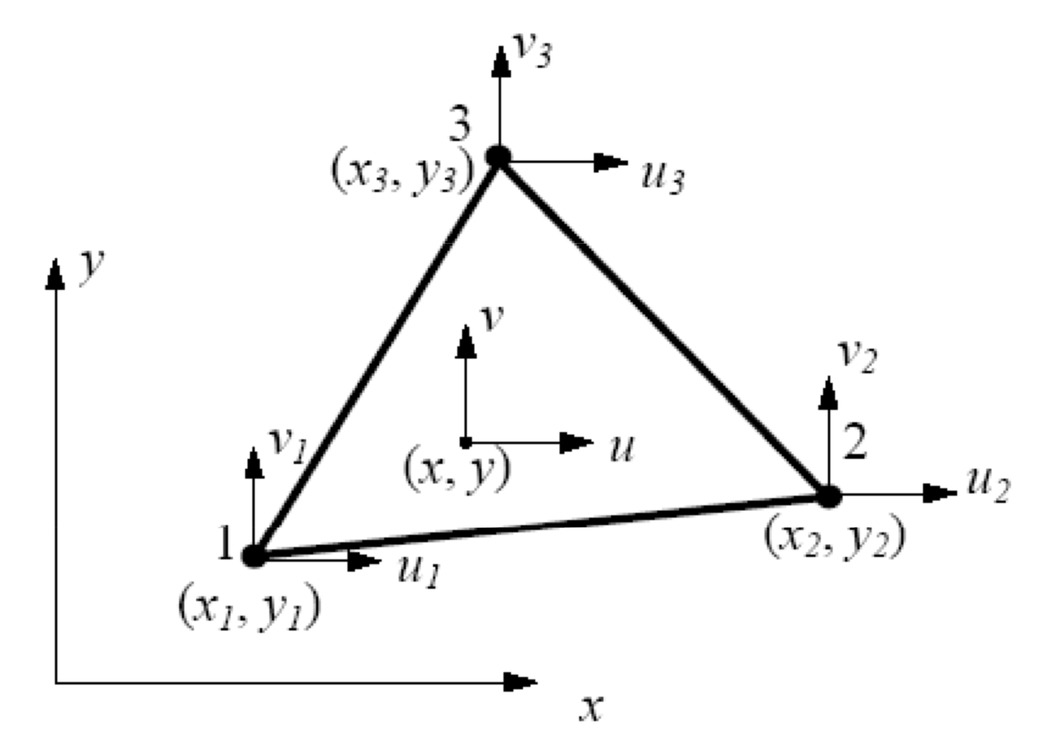
\includegraphics[width=5cm]{images/shapefunctions/triangleFEM1}
\end{center}

For this element, we have three nodes at the vertices of the triangle, which are 
numbered around the element in the counterclockwise direction. 
Each node has two degrees of freedom (can move in the $x$ and $y$ directions). 
The velocities $u$ and $v$ are assumed to be linear functions within the element, that is, 
\[
u=b_1 +b_2x+b_3y
\quad\quad\quad
v=b_4 +b_5x+b_6y
\]
where $b_i$ are constants to be determined and which depend on the triangle shape.
Note that the strain rate components are then given by
\[
\dot\varepsilon_{xx}=b_2 
\quad\quad
\dot\varepsilon_{yy}=b_6 
\quad\quad
\dot\varepsilon_{xy}=(b_3+b_5)/2
\]
and are constant throughout the element.

The velocities should satisfy the following six equations:
\begin{eqnarray}
u_1 &=& b_1 + b_2x_1+b_3y_1 \nn\\
u_2 &=& b_1 + b_2x_2+b_3y_2 \nn\\
u_3 &=& b_1 + b_2x_3+b_3y_3 \nn\\
v_1 &=& b_4 + b_5x_1+b_6y_1 \nn\\
v_2 &=& b_4 + b_5x_2+b_6y_2 \nn\\
v_3 &=& b_4 + b_5x_3+b_6y_3 \nn
\end{eqnarray}

This can be re-written:
\[
\left(
\begin{array}{c}
u_1 \\ u_2 \\ u_3  
\end{array}
\right)
=
\left(
\begin{array}{ccc}
1 & x_1 & y_1 \\
1 & x_2 & y_2 \\
1 & x_3 & y_3 \\
\end{array}
\right)
\cdot
\left(
\begin{array}{c}
b_1 \\ b_2 \\ b_3  
\end{array}
\right)
\]
In order to obtain $b_1,b_2,b_3$ we need to solve this system, or simply to compute the
inverse of the 3x3 ${\bm M}$ matrix, as explained in \ref{sec:inv3x3}.

We define $D=det({\bm M})$ and we get
\[
\left(
\begin{array}{c}
b_1 \\ b_2 \\ b_3  
\end{array}
\right)
=
\frac{1}{D}
\tilde{\bm M}
\cdot
\left(
\begin{array}{c}
u_1 \\ u_2 \\ u_3  
\end{array}
\right)
\]

\[
\left(
\begin{array}{c}
b_4 \\ b_5 \\ b_6  
\end{array}
\right)
=
\frac{1}{D}
\tilde{\bm M}
\cdot
\left(
\begin{array}{c}
v_1 \\ v_2 \\ v_3  
\end{array}
\right)
\]

The matrix $\tilde{\bm M}$ writes:
\[
\tilde{\bm M}
=
\left(
\begin{array}{ccc}
  x_2y_3-x_3y_2  & -(y_3-y_2) &   x_3-x_2 \\
-(x_1y_3-x_3y_1) &   y_3-y_1  & -(x_3-x_1) \\
  x_1y_2-x_2y_1  & -(y_2-y_1) &   x_2-x_1
\end{array}
\right)
\]
ie,
\[
\tilde{\bm M}
=
\left(
\begin{array}{ccc}
x_2y_3-x_3y_2  & y_2-y_3 & x_3-x_2 \\
x_3y_1-x_1y_3  & y_3-y_1 & x_1-x_3 \\
x_1y_2-x_2y_1  & y_1-y_2 & x_2-x_1
\end{array}
\right)
\]
and finally the linear shape functions are given by:
\begin{eqnarray}
N_1(x,y) &=& \frac{1}{D}[(x_2y_3-x_3y_2) + (y_2-y_3)x + (x_3-x_2)y] \nn\\
N_2(x,y) &=& \frac{1}{D}[(x_3y_1-x_1y_3) + (y_3-y_1)x + (x_1-x_3)y] \nn\\
N_3(x,y) &=& \frac{1}{D}[(x_1y_2-x_2y_1) + (y_1-y_2)x + (x_2-x_1)y] \nn
\end{eqnarray}
Note that the area $A$ of the triangle is given by:
\[
A=\frac{1}{2}D = \frac{1}{2}
\left|
\begin{array}{ccc}
1 & x_1 & y_1 \\
1 & x_2 & y_2 \\
1 & x_3 & y_3 
\end{array}
\right|
\]

If we now conder the reference element in the reduced coordinates space $(r,s)$:

\begin{verbatim}
2            
|\
|  \        (r_0,s_0)=(0,0)
|    \      (r_1,s_1)=(1,0)
|      \    (r_2,s_2)=(0,2)
0=======1
\end{verbatim}

The basis polynomial is then
\[
f(r,s) = a + br + cs 
\]
and the shape functions:
\begin{mdframed}[backgroundcolor=blue!5]
\begin{eqnarray}
N_0(r,s) &=& 1-r-s \\
N_1(r,s) &=& r \\
N_2(r,s) &=& s 
\end{eqnarray}
\end{mdframed}

%.....................................................................
\subsubsection{Linear basis functions for quadrilaterals in 2D ($P_1$)}\label{ss:lbfq2D}
\index{general}{$P_1$}

\begin{verbatim}
.=====.=====.
|     |     |
|     3     |   (r_1,s_1)=(0,0)
|     |     |   (r_2,s_2)=(1/2,0)
.=====1==2==.   (r_3,s_3)=(0,1/2)
|     |     |
|     |     |
|     |     |
.=====.=====.
\end{verbatim}

Let us assume that the function $f(r,s)$ is to be approximated on $[-1,1]\times[-1,1]$ by 
\[
f(r,s)=a+br+cs
\]
The function $f$ then must fulfil:
\begin{eqnarray}
f(r_1,s_1)&=&a \;\;\;\;\;\; =f_1    \nn\\
f(r_2,s_2)&=&a+\frac{b}{2}=f_2 \nn\\
f(r_3,s_3)&=&a+\frac{c}{2}=f_3
\end{eqnarray}
This leads to : 
\[
a=f_1
\quad
\quad
b=2(f_2-f_1)
\quad
\quad
c=2(f_3-f_1)
\]
Then
\[
f(r,s)=f_1 + 2(f_2-f_1) r + 2(f_3-f_1) s
\]
or, 
\[
f(r) = \sum_{i=1}^3 N_i(r,s) f_i
\]
with
\begin{mdframed}[backgroundcolor=blue!5]
\begin{eqnarray}
N_1(r) &=& 1-2(r+s)  \nonumber\\
N_2(r) &=& 2r   \nonumber\\
N_3(r) &=& 2s
\end{eqnarray}
\end{mdframed}

Note that we could also have set 
\begin{verbatim}
.=====3=====.
|     |     |
|     |     |   (r_1,s_1)=(0,0)
|     |     |   (r_2,s_2)=(1,0)
.=====1=====2   (r_3,s_3)=(0,1)
|     |     |
|     |     |
|     |     |
.=====.=====.
\end{verbatim}
and we would then have
\begin{mdframed}[backgroundcolor=blue!5]
\begin{eqnarray}
N_1(r) &=& 1-r-s  \nonumber\\
N_2(r) &=& r   \nonumber\\
N_3(r) &=& s
\end{eqnarray}
\end{mdframed}





%.....................................................................
\subsubsection{Enriched linear basis functions in triangles ($P_1^+$)}
\index{general}{$P_1^+$}

As we will see in Section~\ref{pair:mini} the above $P_1$ can be enriched 
with a so-called bubble function.
The \index{general}{Bubble Function} bubble function of the MINI element 
is described in \cite{arbf84} as being $\lambda_1\lambda_2\lambda_3$
where $\lambda_i$ are the so-called barycentric 
coordinates\footnote{\url{https://en.wikipedia.org/wiki/Barycentric\_coordinate\_system }}.
\index{general}{Barycentric Coordinates}

\begin{eqnarray}
\lambda_1 &=& \frac{(y2-y3)(x-x3)+(x3-x2)(y-y3)}{(y2-y3)(x1-x3)+(x3-x2)(y1-y3)} \nn\\
\lambda_2 &=& \frac{(y3-y1)(x-x3)+(x1-x3)(y-y3)}{(y2-y3)(x1-x3)+(x3-x2)(y1-y3)} \nn\\
\lambda_3 &=& 1-\lambda_1-\lambda_2 \nn
\end{eqnarray}

\begin{center}
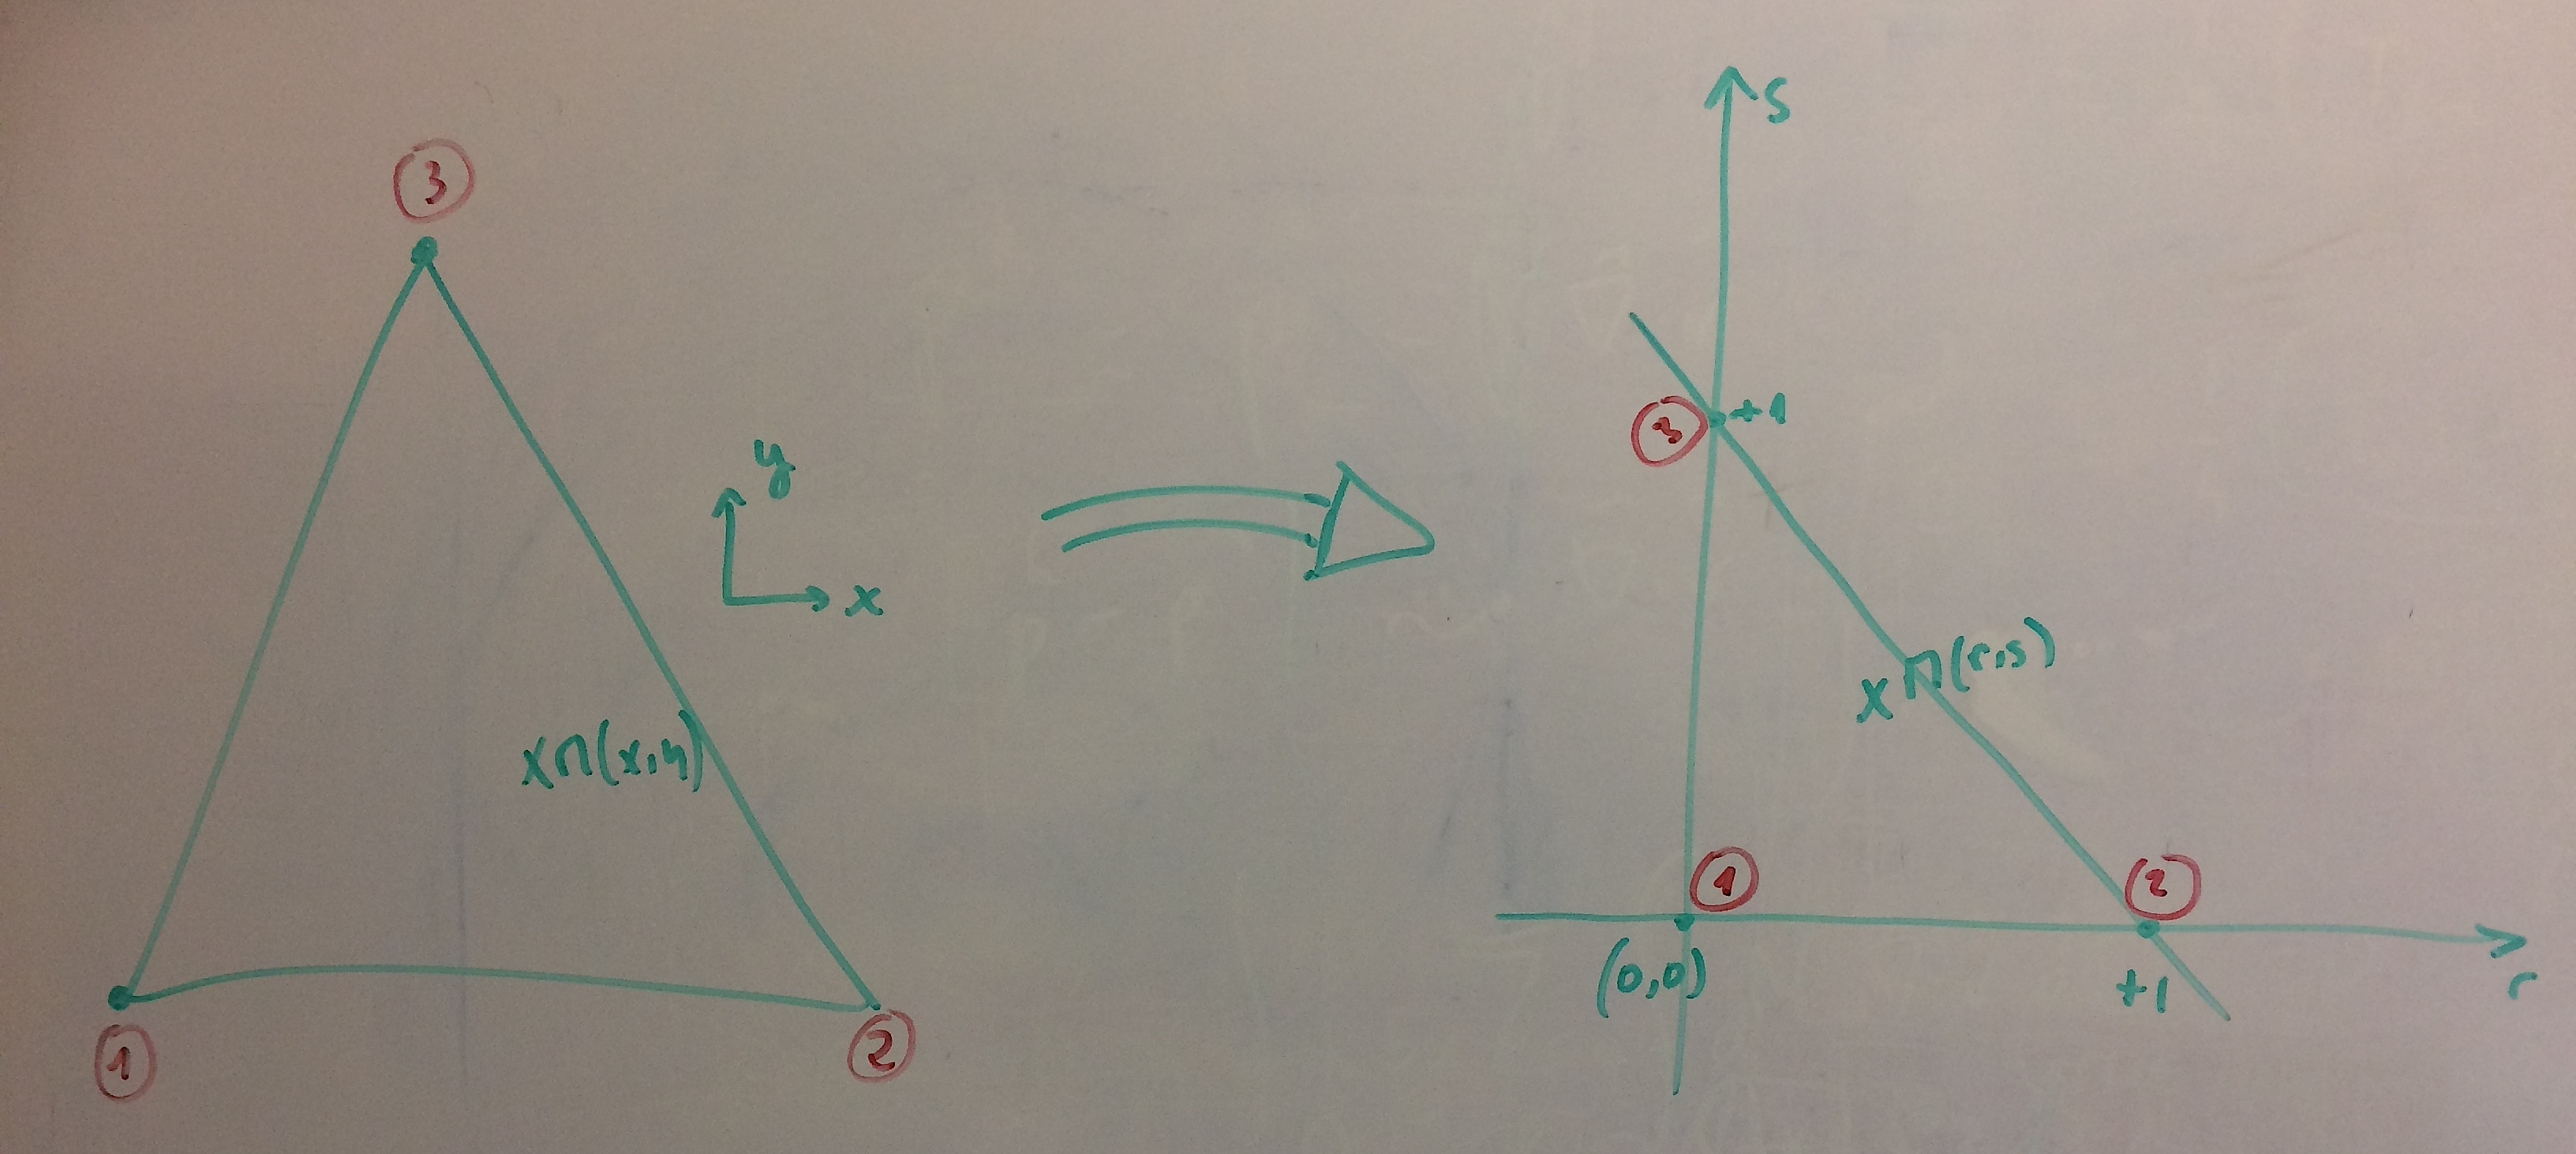
\includegraphics[width=12cm]{images/mini/minielement2}\\
{\small representation of the element in the real coordinate system $(x,y)$
and in the reduced coordinate system $(r,s)$}
\end{center}

\begin{center}
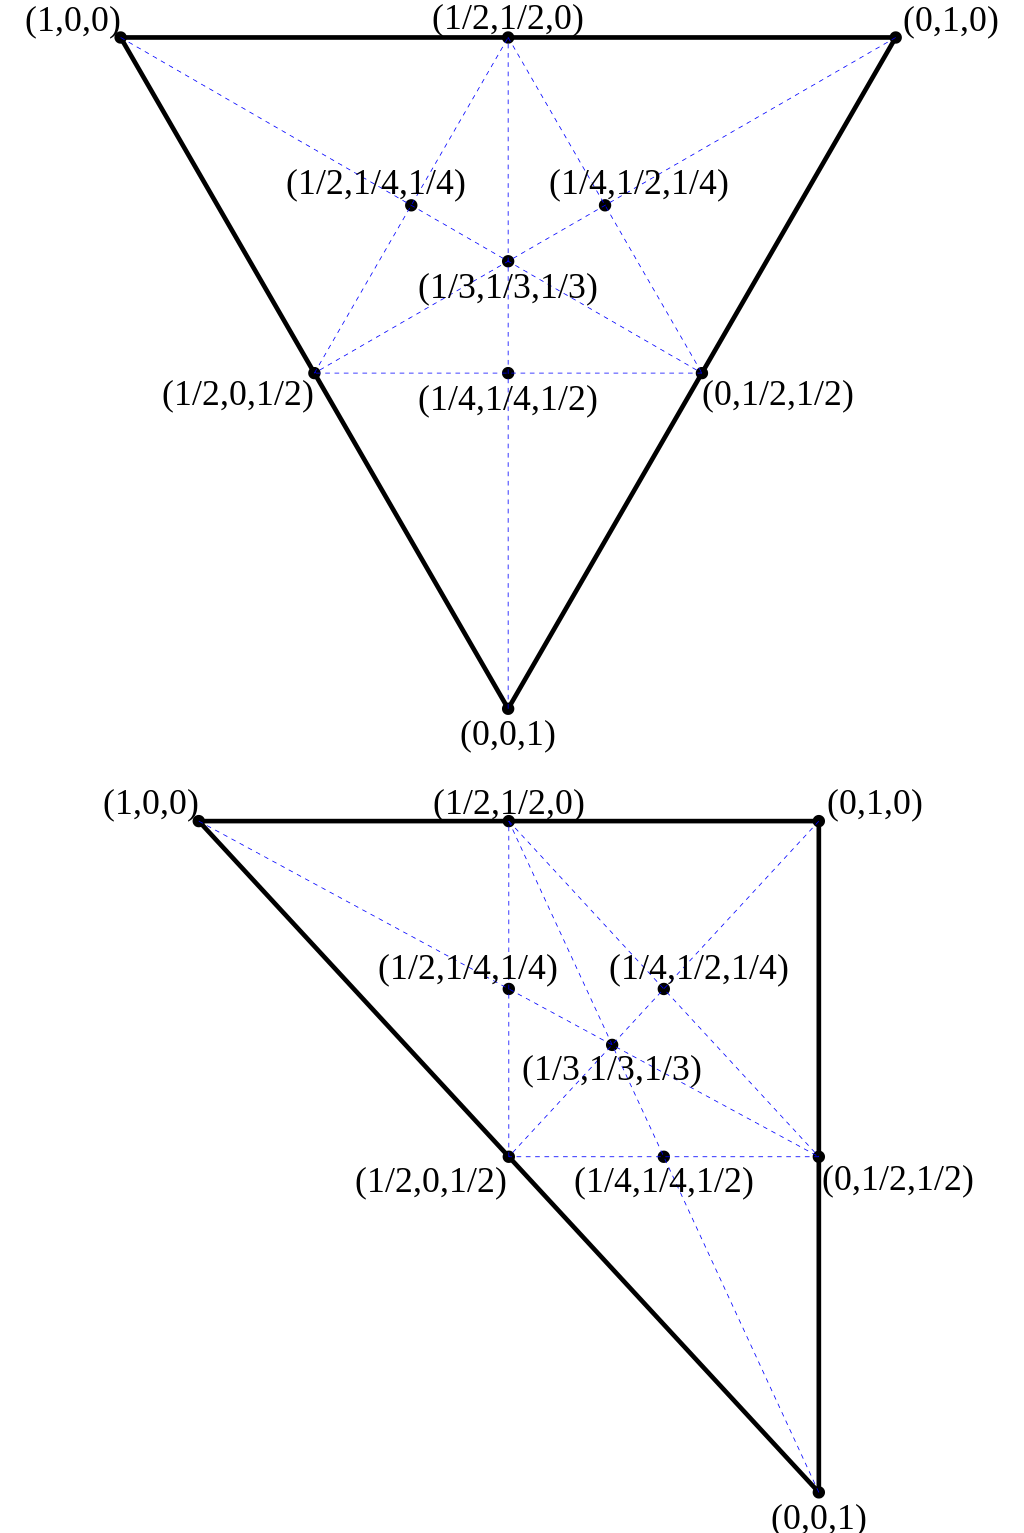
\includegraphics[width=5cm]{images/mini/barycoord}\\
{\small Barycentric coordinates ($\lambda _{1},\lambda _{2},\lambda _{3}$) on an equilateral triangle and on a right triangle.}
\end{center}

In the reference triangle, the barycentric coordinates write
\begin{eqnarray}
\lambda_1 &=& \frac{(s_2-s_3)(r-r_3)+(r_3-r_2)(s-s_3)}{(s_2-s_3)(r_1-r_3)+(r_3-r_2)(s_1-s_3)} = \frac{(-1)(r)+(-1)(s-1)}{(-1)(0)+(-1)(-1)} = -r-s+1  \nn\\
\lambda_2 &=& \frac{(s3-s1)(r-r3)+(r1-r3)(s-s3)}{(s2-s3)(r1-r3)+(r3-r2)(s1-s3)} = \frac{(1)(r)+(0)(s-1)}{(-1)(0)+(-1)(-1)} = r \nn\\
\lambda_3 &=& 1-\lambda_1-\lambda_2 = 1 - (-r-s+1) - r = s \nn
\end{eqnarray}
As we have seen before the bubble function is given by $\lambda_1\lambda_2\lambda_3 = (1-r-s)rs$
and the polynomial form for the shape functions is given by:
\[
f(r,s) =a+br+cs + d (1-r-s)rs
\]
Setting the location of the bubble at $r=s=1/3$, i.e. $\lambda_1\lambda_2\lambda_3 = 1/3$, 
we then have 
\begin{eqnarray}
f(r_1,s_1)&=&f_1 = a+br_1+cs_1 + d (1-r_1-s_1)r_1s_1 = a \nn\\
f(r_2,s_2)&=&f_2 = a+br_2+cs_2 + d (1-r_2-s_2)r_2s_2 = a + b \nn\\
f(r_3,s_3)&=&f_3 = a+br_3+cs_3 + d (1-r_3-s_3)r_3s_3 = a + c \nn\\
f(r_4,s_4)&=&f_4 = a+br_4+cs_4 + d (1-r_4-s_4)r_4s_4 = a + \frac{b}{3} + \frac{c}{3} + \frac{1}{27} \nn
\end{eqnarray}
where point 4 is the location of the bubble.
This yields
\[
a=f_1 
\quad\quad\qquad
b=f_2-a = f_2-f_1
\quad\quad\qquad
c=f_3-a = f_3-f_1
\]
and
\[
d=27(f_4-a-\frac{b}{3} - \frac{c}{3}) = 27 (f_4 - f_1 - \frac{f_2-f_1}{3} - \frac{f_3-f_1}{3} )
=27(f_4 - \frac{f_1}{3}  - \frac{f_2}{3}  - \frac{f_3}{3} )
\] 

Finally
\begin{eqnarray}
f(r,s) 
&=&a+br+cs + d (1-r-s)rs \nn\\
&=& f_1 + (f_2-f_1)r + (f_3-f_1)s + 27(f_4 - \frac{f_1}{3}  - \frac{f_2}{3}  - \frac{f_3}{3} ) (1-r-s)rs \nn\\
&=& [1-r-s-9(1-r-s)rs] f_1 + [r-9(1-r-s)rs ]f_2 + [s-9(1-r-s)rs ]f_3 + [27(1-r-s)rs]f_4 \nn
\end{eqnarray}
so that 
\[
f(r,s)=\sum_{i=1}^4 N_i(r,s) f_i
\]
with 
%\begin{mdframed}[backgroundcolor=blue!15]
\begin{eqnarray}
N_1(r,s) &=& 1-r-s-9(1-r-s)rs \nn\\
N_2(r,s) &=& r-9(1-r-s)rs \nn\\
N_3(r,s) &=& s-9(1-r-s)rs \nn\\
N_4(r,s) &=& 27(1-r-s)rs \nn
\end{eqnarray}
%\end{mdframed}
It is trivial to verify that $\sum_i N_i =1$ for all values of $r,s$
and the gradients of the shape functions are:
\begin{eqnarray}
\frac{\partial N_1}{\partial r}(r,s) &=& -1 - 9(1-2r-s)s \\ 
\frac{\partial N_2}{\partial r}(r,s) &=&  +1 - 9(1-2r-s)s \\ 
\frac{\partial N_3}{\partial r}(r,s) &=&  - 9(1-2r-s)s \\ 
\frac{\partial N_4}{\partial r}(r,s) &=&  27(1-2r-s)s \\ 
\\
\frac{\partial N_1}{\partial s}(r,s) &=& -1 - 9(1-r-2s)r \\ 
\frac{\partial N_2}{\partial s}(r,s) &=&    - 9(1-r-2s)r \\ 
\frac{\partial N_3}{\partial s}(r,s) &=& +1 - 9(1-r-2s)r \\ 
\frac{\partial N_4}{\partial s}(r,s) &=&     27(1-r-2s)r 
\end{eqnarray}

We have two coordinate systems for the element: the global coordinates $(x,y)$ 
and the natural coordinates $(r,s)$. Inside the element, the relation between the two is given by
\begin{eqnarray}
x &=& N_1 x_1 + N_2 x_2 + N_3 x_3 + N_4 x_4 = \sum_i N_i(r,s) x_i\nn\\
y &=& N_1 y_1 + N_2 y_2 + N_3 y_3 + N_4 y_4 = \sum_i N_i(r,s) y_i
\end{eqnarray}
or,
\begin{eqnarray}
x &=& [ 1-r-s-9(1-r-s)rs] x_1 + [r-9(1-r-s)rs] x_2 + [s-9(1-r-s)rs] x_3 + [27(1-r-s)rs] x_4 \nn\\
&=& x_1 -r (x_1-x_2) -s (x_1-x_3) + (1-r-s)rs (-9 x_1 - 9 x_2  -9 x_3 +27 x_4)  \nn\\
&=& x_1 -r (x_1-x_2) -s (x_1-x_3) + (1-r-s)rs (-9 x_1 - 9 x_2  -9 x_3 +27 (x_1+x_2+x_3)/3) \nn\\ 
&=& x_1 -r (x_1-x_2) -s (x_1-x_3) \nn\\ 
&=& x_1 -r x_{12} -s x_{13} \nn\\ 
y &=& [ 1-r-s-9(1-r-s)rs] y_1 + [r-9(1-r-s)rs] y_2 + [s-9(1-r-s)rs] y_3 + [27(1-r-s)rs] y_4 \nn\\
&=& y_1 -r (y_1-y_2) -s (y_1-y_3) + (1-r-s)rs (-9 y_1 - 9 y_2  -9 y_3 +27 y_4)  \nn\\
&=& y_1 -r (y_1-y_2) -s (y_1-y_3) + (1-r-s)rs (-9 y_1 - 9 y_2  -9 y_3 +27 (y_1+y_2+y_3)/3) \nn\\ 
&=& y_1 -r (y_1-y_2) -s (y_1-y_3) \nn \\
&=& y_1 -r y_{12} -s y_{13} \nn 
\end{eqnarray}




























%%%%%%%%%%%%%%%%%%%%%%%%%%%%%%%%%%%%
\subsubsection{Quadratic basis functions for triangles in 2D ($P_2$)}
\index{general}{$P_2$}

\begin{verbatim}
2            
|\
| \        (r_0,s_0)=(0,0) (r_3,s_3)=(1/2,0)
5   4      (r_1,s_1)=(1,0) (r_4,s_4)=(1/2,1/2)
|     \    (r_2,s_2)=(0,1) (r_5,s_5)=(0,1/2)
|      \ 
0===3===1
\end{verbatim}
The basis polynomial is then
\[
f(r,s) = c_1 + c_2 r + c_3 s + c_4  r^2 + c_5 rs  + c_6 s^2
\]
We have 
\begin{eqnarray}
f_1 = f(r_1,s_1) &=& c_1 \nonumber\\
f_2 = f(r_2,s_2) &=& c_1 + c_2 + c_4\nonumber\\
f_3 = f(r_3,s_3) &=& c_1 + c_3 + c_6\nonumber\\
f_4 = f(r_4,s_4) &=& c_1 + c_2/2 + c_4/4\nonumber\\
f_5 = f(r_5,s_5) &=& c_1 + c_2/2 + c_3/2 \nonumber\\
                 &+& c_4/4 + c_5/4 + c_6/4\nonumber\\
f_6 = f(r_6,s_6) &=& c_1 + c_3/2 + c_6/4\nonumber
\end{eqnarray}

This can be cast as ${\bm f}={\bm A}\cdot {\bm c}$ where ${\bm A}$ is a 6x6 matrix:
\[
{\bm A}=
\left(
\begin{array}{cccccc}
1&0   &  0  & 0   & 0   & 0\\
1&1   &  0  & 1   & 0   & 0\\
1&0   &  1  & 0   & 0   & 1\\
1&1/2 &  0  & 1/4 & 0   & 0\\
1&1/2 &  1/2& 1/4 & 1/4 & 1/4\\
1&0   &  1/2& 0   & 0   & 1/4
\end{array}
\right)
\]
It is rather trivial to compute the inverse of this matrix:
\[
{\bm A}^{-1}=
\left(
\begin{array}{cccccc}
1  & 0 & 0  & 0  & 0 & 0  \\
-3 & -1& 0  & 4  & 0 & 0 \\
-3 & 0 & -1 & 0  & 0 & 4 \\
2  & 2 & 0  & -4 & 0 & 0  \\
4  & 0 & 0  & -4 & 4 & -4 \\
2  & 0 & 2  & 0  & 0 & -4
\end{array}
\right)
\]
In the end, one obtains:
\begin{eqnarray}
f(r,s) 
&=& f_1 + (-3f_1-f_2+4f_4) r + (-3f_1-f_3+4f_6)s \nonumber\\
&& +(2f_1+2f_2-4f_4)r^2 + (4f_1-4f_4+4f_5-4f_6) rs \nn\\
&&+ (2f_1+2f_3-4f_6)s^2 \nonumber\\
&=& \sum_{i=1}^6 N_i(r,s) f_i
\end{eqnarray}
with
\begin{mdframed}[backgroundcolor=blue!5]
\begin{eqnarray}
N_1(r,s) &=& 1-3r-3s+2r^2+4rs+2s^2 \nonumber\\
N_2(r,s) &=& -r+2r^2 \nonumber\\
N_3(r,s) &=& -s+2s^2 \nonumber\\
N_4(r,s) &=& 4r-4r^2-4rs \nonumber\\
N_5(r,s) &=& 4rs \nonumber\\
N_6(r,s) &=& 4s-4rs-4s^2 \nonumber
\end{eqnarray}
\end{mdframed}


%.....................................................................
\subsubsection{Enriched quadratic basis functions in triangles ($P_2^+$)}
\index{general}{$P_2^+$}

This is used by the Crouzeix-Raviart element, see Section~\ref{sec:crouzeix-raviart}. 
\index{general}{Crouzeix-Raviart}

\begin{verbatim}
03             (r_1,s_1)=(0,0)
||\\           (r_2,s_2)=(1,0)
|| \\          (r_3,s_3)=(0,1)
||  \\         (r_4,s_4)=(1/2,0)
06   05        (r_5,s_5)=(1/2,1/2)
|| 07 \\       (r_6,s_6)=(0,1/2)
||     \\      (r_7,s_7)=(1/3,1/3)
01==04==02    
\end{verbatim}

The shape functions are given by:
\todo[inline]{find reference}

\begin{mdframed}[backgroundcolor=blue!5]
\begin{eqnarray}
N_1(r,s) &=&  (1-r-s)(1-2r-2s+ 3rs) \\
N_2(r,s) &=& r (2 r -1 + 3s-3rs-3s^2 ) \\
N_3(r,s) &=& s (2s -1 + 3r-3r^2-3rs )\\
N_4(r,s) &=& 4(1-r-s)r(1 -3s ) \\
N_5(r,s) &=& 4rs [-2+3r+3s]\\
N_6(r,s) &=& 4(1-r-s)s(1-3r)\\
N_7(r,s) &=& 27 (1-r-s)rs 
\end{eqnarray}
\end{mdframed}
It is then easy to verify that for all shape functions we have 
$N_i(r_j,s_j)=\delta_{ij}$ where $j$ denotes one of the seven nodes. 

The derivatives are as follows:
\begin{eqnarray}
\frac{\partial N_1}{\partial r}(r,s) &=& r(4-6s)-3s^2+7s-3\\
\frac{\partial N_2}{\partial r}(r,s) &=& r(4-6s)-3s^2+3s-1\\
\frac{\partial N_3}{\partial r}(r,s) &=& -3s(2r+s-1)  \\
\frac{\partial N_4}{\partial r}(r,s) &=& 4(3s-1)(2r+s-1) \\
\frac{\partial N_5}{\partial r}(r,s) &=& 4s(6r+3s-2) \\
\frac{\partial N_6}{\partial r}(r,s) &=& 4s(6r+3s-4)\\
\frac{\partial N_7}{\partial r}(r,s) &=& -27s(2r+s-1)
\end{eqnarray}

\begin{eqnarray}
\frac{\partial N_1}{\partial s}(r,s) &=& -3r^2+r(7-6s)+4s-3\\
\frac{\partial N_2}{\partial s}(r,s) &=& -3r(r+2s-1)\\
\frac{\partial N_3}{\partial s}(r,s) &=& -3r^2+r(3-6s)+4s-1 \\
\frac{\partial N_4}{\partial s}(r,s) &=& 4r(3r+6s-4)  \\
\frac{\partial N_5}{\partial s}(r,s) &=& 4r(3r+6s-2) \\
\frac{\partial N_6}{\partial s}(r,s) &=& 4(3r-1)(r+2s-1)\\
\frac{\partial N_7}{\partial s}(r,s) &=& -27r(r+2s-1)
\end{eqnarray}


Note that the shape functions can also be expressed as a function of the barycentric coordinates, 
as in the MILAMIN code \cite{daks08} or in Cuvelier et al, 1986 \cite{cuss86}\footnote{Note
that the numbering of the nodes in the book is different with respect to the one above. }

\begin{verbatim}
03          
||\\        
|| \\       
||  \\      
05   04     
|| 07 \\    
||     \\   
01==06==02    
\end{verbatim}

\begin{eqnarray}
N_1(\lambda_1,\lambda_2,\lambda_3) &=& \eta_1(2\eta_1-1)+ 3\eta_1\eta_2\eta_3\\
N_2(\lambda_1,\lambda_2,\lambda_3) &=& \eta_2(2\eta_2-1)+ 3\eta_1\eta_2\eta_3\\
N_3(\lambda_1,\lambda_2,\lambda_3) &=& \eta_3(2\eta_3-1)+ 3\eta_1\eta_2\eta_3\\
N_4(\lambda_1,\lambda_2,\lambda_3) &=& 4\eta_2\eta_3 - 12\eta_1\eta_2\eta_3\\
N_5(\lambda_1,\lambda_2,\lambda_3) &=& 4\eta_1\eta_3 - 12\eta_1\eta_2\eta_3\\
N_6(\lambda_1,\lambda_2,\lambda_3) &=& 4\eta_1\eta_2 - 12\eta_1\eta_2\eta_3\\
N_7(\lambda_1,\lambda_2,\lambda_3) &=& 27\eta_1\eta_2\eta_3 
\end{eqnarray}

\todo[inline]{
VERIFY that when $\eta_1=1-r-s$, $\eta_2=r$ and $\eta_3=s$ we find the above $r,s$ shape functions
}


%1-4*eta1+3*eta1*eta3-3*eta2*eta3 ...
%-1+4*eta2+3*eta1*eta3-3*eta2*eta3 ...
%3*eta1*eta3-3*eta2*eta3 ...
%4*eta3+12*eta2*eta3-12*eta1*eta3 ...
%-4*eta3+12*eta2*eta3-12*eta1*eta3 ...
%4*eta1-4*eta2+12*eta2*eta3-12*eta1*eta3 ...
%-27*eta2*eta3+27*eta1*eta3

%1-4*eta1+3*eta1*eta2-3*eta2*eta3 ...
%+3*eta1*eta2-3*eta2*eta3 ...
%-1+4*eta3+3*eta1*eta2-3*eta2*eta3 ...
%4*eta2-12*eta1*eta2+12*eta2*eta3 ...
%4*eta1-4*eta3-12*eta1*eta2+12*eta2*eta3 ...
%-4*eta2-12*eta1*eta2+12*eta2*eta3 ...
%27*eta1*eta2-27*eta2*eta3];  







%%%%%%%%%%%%%%%%%%%%%%%%%%%%%%%%%%%%
\subsubsection{Cubic basis functions for triangles ($P_3$)}
\index{general}{$P_3$}

\begin{verbatim}
2
|\          (r_0,s_0)=(0,0)   (r_5,s_5)=(2/3,1/3)
|  \        (r_1,s_1)=(1,0)   (r_6,s_6)=(1/3,2/3)
7   6       (r_2,s_2)=(0,1)   (r_7,s_7)=(0,2/3)
|    \      (r_3,s_3)=(1/3,0) (r_8,s_8)=(0,1/3)
8  9   5    (r_4,s_4)=(2/3,0) (r_9,s_9)=(1/3,1/3)
|       \ 
0==3==4==1
\end{verbatim}
The basis polynomial is then
\[
f(r,s) = c_1 + c_2r + c_3s + c_4 r^2 + c_5 rs + c_6 s^2 + c_7 r^3 +c_8 r^2s + c_9 rs^2 + c_{10}s^3
\]
\begin{eqnarray}
N_0(r,s) &=& \frac{9}{2}(1-r-s)(1/3-r-s)(2/3-r-s) \\
N_1(r,s) &=& \frac{9}{2}r(r-1/3)(r-2/3) \\
N_2(r,s) &=& \frac{9}{2}s(s-1/3)(s-2/3) \\
N_3(r,s) &=& \frac{27}{2}(1-r-s)r(2/3-r-s) \\
N_4(r,s) &=& \frac{27}{2}(1-r-s)r(r-1/3) \\
N_5(r,s) &=& \frac{27}{2}rs(r-1/3) \\
N_6(r,s) &=& \frac{27}{2}rs(r-2/3) \\
N_7(r,s) &=& \frac{27}{2}(1-r-s)s(s-1/3) \\
N_8(r,s) &=& \frac{27}{2}(1-r-s)s(2/3-r-s) \\
N_9(r,s) &=& 27 rs(1-r-s)
\end{eqnarray}
\todo[inline]{verify those}




















%..........................................................................
\subsubsection{Enriched linear basis functions in quadrilaterals ($Q_1^+$) -WIP} \label{ss:quadmini}
\index{general}{$Q_1^+$}

\begin{verbatim}
4===========3
|           |   (r_1,s_1)=(-1,-1)
|           |   (r_2,s_2)=(1,-1)
|     5     |   (r_3,s_3)=(1,1)
|           |   (r_4,s_4)=(-1,1)
|           |   (r_5,s_5)=(0,0)
1===========2
\end{verbatim}

In Bai (1997) \cite{bai97}: "It is well known that the equal-order bilinear velocity-bilinear 
continuous pressure element - the $Q_1\times Q_1$, element - exhibits a certain spurious pressure mode.
In the paper we propose a new stabilized Q1Q1 combination for the velocity and
pressure with three internal degrees of freedom added to the velocity space, that is, one degree of
freedom for each component of the velocity and one degree of freedom shared by both components of
the velocity."

Two versions are proposed, if I understand it correctly.
The first one is given in Eq.7 (three extra dofs: $u_5$, $v_5$, $w$):
\begin{eqnarray}
u(r,t) &=& \sum_{i=1}^4 N_i (r,t) u_i + \left[ u_5 - \frac{w}{4}(1-t) \right] (1-r^2)(1-t^2) \nonumber\\
v(r,t) &=& \sum_{i=1}^4 N_i (r,t) v_i + \left[ v_5 - \frac{w}{4}(1-r) \right] (1-r^2)(1-t^2) 
\end{eqnarray}
The second one in Eq.23 (four extra dofs: $u_5$, $v_5$, $u_6$, $v_6$):
\begin{eqnarray}
u(r,t) &=& \sum_{i=1}^4 N_i (r,t) u_i + \left[ u_5 +u_6(r+t) \right] (1-r^2)(1-t^2) \nonumber\\
v(r,t) &=& \sum_{i=1}^4 N_i (r,t) v_i + \left[ v_5 +v_6(r+t) \right] (1-r^2)(1-t^2) 
\end{eqnarray}

In Franca et al (2007) \cite{fros07}: 
stabilized finite element method for Stokes equations with piecewise continuous 
bilinear approximations for both velocity and pressure variables. The velocity
field is enriched with piecewise polynomial bubble functions with null average at element
edges.

In Kwon \& Park \cite{kwpa14}: 
"We introduce a new stable MINI-element pair for incompressible Stokes equations on
quadrilateral meshes, which uses the smallest number of bubbles for the velocity. The pressure is 
discretized with the $P_1$ -midpoint-edge-continuous elements and each component of the velocity field is
done with the standard $Q_1$ -conforming elements enriched by one bubble a quadrilateral."


In Lamichhane (2017) \cite{lami17}: "We consider a quadrilateral MINI
finite element for approximating the solution
of Stokes equations using a quadrilateral mesh. We use the standard bilinear finite
element space enriched with element-wise defined bubble functions for the velocity
and the standard bilinear finite element space for the pressure space. With a simple
modification of the standard bubble function we show that a single bubble function is
sufficient to ensure the inf-sup condition.
This is a refinement of \cite{bai97} where the author enriches the velocity space with
more than a single vector bubble function per element. In this article we show that with a small modification of the standard bubble function we can get the stability just by using a single vector bubble function per element."

The two bubble functions are defined on the reference element $[-1,1]\times [-1,1]$:
\begin{eqnarray}
b^{(1)}(x,y) &=&  (1-r)(1-s)\cdot (1-r^2) (1-s^2) \\  
b^{(2)}(x,y) &=&  \left(1+\frac{r+s}{4}\right) \cdot (1-r^2) (1-s^2) 
\end{eqnarray}
Both bubble functions are exactly one in the middle of the element and exactly zero on the edges
of the element as expected from shape functions.


%In what follows I focus on the two bubble functions $b^{(1)}$ and $b^{(2)}$ in \cite{lami17}.
%When I rewrite these for the reference element $[-1,1]\times[-1,1]$, then $x=(r+1)/2$, $y=(s+1)/2$
%and $1-x=(1-r)/2$ and $1-y=(1-s)/2$.
%\begin{eqnarray}
%b^{(1)}(r,s) 
%&=& 64 \frac{1}{4} (1-r)^2 \frac{1}{4}(1-s)^2 \frac{1}{2} (r+1) \frac{1}{2} (s+1)  \\
%&=&  (1-r)^2 (1-s)^2 (r+1)  (s+1) \\
%&=& (1-r)(1-s) (1-r^2) (1-s^2) \\ \nn\\ 
%b^{(2)}(r,s) 
%&=& 8[1+(r+1)/2+(s+1)/2]\frac{1}{2}(r+1)\frac{1}{2}(s+1)\frac{1}{2}(1-r)\frac{1}{2}(1-s) \\
%&=& \frac{1}{2} [1+(r+1)/2+(s+1)/2] (r+1) (s+1) (1-r) (1-s) \\
%&=& \left(1+\frac{r+s}{4}\right) (1-r^2) (1-s^2) 
%\end{eqnarray}

We then have
\begin{eqnarray}
\frac{\partial b^{(1)}}{\partial r}(r,s) 
&=& (1-s)^2(1+s)[-2(1-r)(1+r)+(1-r)^2]\\
&=& (1-s)^2(1+s)[-2+2r^2 + 1-2r+r^2]\\
&=& (1-s)^2(1+s)[-1-2r+3r^2]\\
\frac{\partial b^{(1)}}{\partial s}(r,s) 
&=& (1-r)^2(1+r)[-1-2s+3s^2 ] \\
\frac{\partial b^{(2)}}{\partial r}(r,s) 
&=& \frac{1}{4} (1-s^2) (1-r^2 + (4+r+s) (-2r)) \\
&=& \frac{1}{4} (1-s^2) (1-8r-3r^2 -2rs) \\
\frac{\partial b^{(2)}}{\partial s}(r,s) 
&=& \frac{1}{4} (1-r^2) (1-s^2 + (4+r+s) (-2s)) \\
&=& \frac{1}{4} (1-r^2) (1-8s-3s^2 -2rs) 
\end{eqnarray}
We postulate that a function $f$ has the following representation 
in the element:
\[
f^h(r,s)=a+br+cs+drs+e b(r,s) 
\]
where $b(r,s)$ stands for the bubble function which is of the form $b(r,s)=(1-r^2)(1-s^2)\phi(r,s)$
and $\phi$ is a (bi)-linear function of $r,s$.

We need
\begin{eqnarray}
f^h(r_1,s_1) &=& a-b-c+d  =f_1 \\
f^h(r_2,s_2) &=& a+b-c-d  =f_2 \\
f^h(r_3,s_3) &=& a+b+c+d  =f_3 \\
f^h(r_4,s_4) &=& a-b+c-d  =f_4 \\
f^h(r_5,s_5) &=& a      +e=f_5 
\end{eqnarray}
This can be written as a linear system: 
\[
\left(
\begin{array}{ccccc}
1 &-1 &-1 & 1 &0 \\
1 & 1 &-1 &-1 &0 \\
1 & 1 & 1 & 1 &0 \\
1 &-1 & 1 &-1 &0 \\
1 & 0 & 0 & 0 &1 
\end{array}
\right)
\cdot
\left(
\begin{array}{c}
a \\ b \\ c \\ d \\ e
\end{array}
\right)
=
\left(
\begin{array}{c}
f_1 \\ f_2 \\ f_3 \\ f_4 \\ f_5
\end{array}
\right)
\]
and the solution is then:
\[
\left(
\begin{array}{c}
a \\ b \\ c \\ d \\ e
\end{array}
\right)
=
\frac{1}{4}
\left(
\begin{array}{ccccc}
 1 & 1 &  1 & 1 &0\\
-1 & 1 &  1 &-1 &0\\
-1 &-1 &  1 & 1 &0\\
 1 &-1 &  1 &-1 &0\\
-1 &-1 & -1 &-1 &4
\end{array}
\right)
\cdot
\left(
\begin{array}{c}
f_1 \\ f_2 \\ f_3 \\ f_4 \\ f_5
\end{array}
\right)
\]
or, 
\begin{eqnarray}
a &=& \frac{1}{4}( f_1 + f_2 +f_3 +f_4) \\
b &=& \frac{1}{4}(-f_1 + f_2 +f_3 -f_4) \\
c &=& \frac{1}{4}(-f_1 - f_2 +f_3 +f_4) \\
d &=& \frac{1}{4}( f_1 - f_2 +f_3 -f_4) \\
e &=& \frac{1}{4}(-f_1 - f_2 -f_3 -f_4 + 4f_5) 
\end{eqnarray}
Then 
\begin{eqnarray}
4f^h(r,s)
&=&4 [a+br+cs+drs+e (1-r^2) (1-s^2) \phi(r,s)] \\
&=&  (f_1 + f_2 +f_3 +f_4) \\
&+& (-f_1 + f_2 +f_3 -f_4)r \\
&+&(-f_1 - f_2 +f_3 +f_4)s \\
&+& (f_1 - f_2 +f_3 -f_4)rs \\
&+& (-f_1 - f_2 -f_3 -f_4 + 4f_5) (1-r^2) (1-s^2) \phi(r,s) \\
&=& (1-r-s+rs - b(r,s))f_1 \\
&+& (1+r-s-rs-b(r,s))f_2 \\
&+& (1+r+s+rs-b(r,s))f_3 \\
&+& (1-r+s-rs- b(r,s))f_4 \\
&+& 4b(r,s) f_5
\end{eqnarray}
or, 

\begin{eqnarray}
f^h(r,s)&=&
\underbrace{\left(\frac{1}{4}(1-r)(1-s)-\frac{1}{4}b(r,s)\right)}_{N_1} f_1 + 
\underbrace{\left(\frac{1}{4}(1+r)(1-s)-\frac{1}{4}b(r,s)\right)}_{N_2} f_2\\
&+& 
\underbrace{\left(\frac{1}{4}(1+r)(1+s)-\frac{1}{4}b(r,s)\right)}_{N_3} f_3 +
\underbrace{\left(\frac{1}{4}(1-r)(1+s)-\frac{1}{4}b(r,s)\right)}_{N_4} f_4 \\
&+& \underbrace{b(r,s)}_{N_5} f_5
\end{eqnarray}

As in the $P_1^+$ case the resulting shape functions are a combination 
of the regular $Q_1$ shape functions and the bubble.


Consistency check $f(r,s)=C$:
\begin{eqnarray}
f^h(r,s) 
&=& \sum_{i=1}^5 N_i(r,s) f_i \\
&=& C \sum_{i=1}^5 N_i(r,s)  \\
&=& C
\end{eqnarray}

Consistency check $f(r,s)=r$ (or $f(r,s)=s)$:
\begin{eqnarray}
f^h(r,s) 
&=& \sum_{i=1}^5 N_i(r,s) f_i \\
&=& N_1 (-1) + N_2 (+1) + N_3 (+1) + N_4 (-1) + N_5 (0) \\
&=& -N_1+N_2+N_3-N_4 \\
&=& r
\end{eqnarray}

Consistency check $f(r,s)=rs$ ($f_1=(-1)(-1)=1$, $f_2=(+1)(-1)=-1$, etc ...)
\begin{eqnarray}
f^h(r,s) 
&=& \sum_{i=1}^5 N_i(r,s) f_i \nn\\
&=& N_1 (+1) + N_2 (-1) + N_3 (+1) + N_4 (-1) + N_5 (0) \nn\\
&=& N_1-N_2+N_3-N_4 \nn\\
&=& 
\left(\frac{1}{4}(1-r)(1-s)-\frac{1}{4}b(r,s)\right)
-\left(\frac{1}{4}(1+r)(1-s)-\frac{1}{4}b(r,s)\right) \nn\\
&+& 
\left(\frac{1}{4}(1+r)(1+s)-\frac{1}{4}b(r,s)\right)
-\left(\frac{1}{4}(1-r)(1+s)-\frac{1}{4}b(r,s)\right) \nn\\
&=& 
 \frac{1}{4}(1-r)(1-s)
-\frac{1}{4}(1+r)(1-s)
+\frac{1}{4}(1+r)(1+s)
-\frac{1}{4}(1-r)(1+s) \nn\\
&=&
 \frac{1}{2}(-r)(1-s)
+\frac{1}{2}(+r)(1+s) \nn\\
&=& rs
\end{eqnarray}

We find that the shape functions can represent  a bilinear field exactly. 
Let us now turn to quadratic terms:

Consistency check $f(r,s)=r^2$ (or $f(r,s)=s^2$): 
\begin{eqnarray}
f^h(r,s) 
&=& \sum_{i=1}^5 N_i(r,s) f_i \nn\\
&=& N_1(r,s)\cdot (+1) + N_2(r,s)\cdot (+1) + N_3(r,s)\cdot (+1) + N_4(r,s)\cdot (+1) + N_5(r,s)\cdot (0) \nn\\
&=& 
\left(\frac{1}{4}(1-r)(1-s)-\frac{1}{4}b(r,s)\right)
+\left(\frac{1}{4}(1+r)(1-s)-\frac{1}{4}b(r,s)\right) \nn\\
&+& 
\left(\frac{1}{4}(1+r)(1+s)-\frac{1}{4}b(r,s)\right)
+\left(\frac{1}{4}(1-r)(1+s)-\frac{1}{4}b(r,s)\right) \nn\\
&=&
\frac{1}{2}(1-s) + \frac{1}{2}(1+s) -b(r,s) \nn\\
&=& 
1 - b(r,s) 
\end{eqnarray}

We have 
\begin{eqnarray}
\int_{-1}^{+1} \int_{-1}^{+1} (1-b_1(r,s)) dr ds  
&=& \int_{-1}^{+1} \int_{-1}^{+1} [1 - (1-r^2)(1-s^2)(1-r)(1-s) ] dr ds = 20/9 \simeq 2.2222 \nn\\
\int_{-1}^{+1} \int_{-1}^{+1} (1-b_2(r,s,\beta)) dr ds  
&=& \int_{-1}^{+1} \int_{-1}^{+1} [1 - (1-r^2)(1-s^2)(1+\beta(r+s)) ] dr ds = 20/9  \qquad \forall \beta \nn 
\end{eqnarray}
Both bubbles yield the same average. This is not helpful. 

Let us now look at the (root) mean square:
\begin{eqnarray}
\int_{-1}^{+1} \int_{-1}^{+1} (1-b_1(r,s))^2 dr ds &=& 21284/11025 \simeq 1.93052 \nn\\
\int_{-1}^{+1} \int_{-1}^{+1} (1-b_2(r,s,\beta))^2 dr ds &=& \frac{4}{1575} (128 \beta^2  + 623) 
\end{eqnarray}
The problem is that the minimum is reached for $\beta=0$ which is not allowed so 
we cannot choose $\beta$ so as to minimise the error.
For $\beta=0.25$ as used in the paper:
\[
\int_{-1}^{+1} \int_{-1}^{+1} (1-b_2(r,s))^2 dr ds = 2524/1575 \simeq 1.60254 
\]
On the other hand, this means that using the second bubble function does a better job  
at representing square terms ($r^2$, $s^2$) than using the first one. 




\newpage
One can also revisit the second bubble function: in Lamichhane (2017) \cite{lami17}
it is postulated to be defined by 
\begin{eqnarray}
b^{(2)}(r,s) &=& (a+br+cs)(1-r^2)(1-s^2) \qquad abc\neq 0
\end{eqnarray}
on the reference element $[-1,1]\times [-1,1]$. Then the author 
states that 'for simplicity we choose':
\begin{eqnarray}
b^{(2)}(r,s) &=& \frac{1}{4} (4+r+s)(1-r^2)(1-s^2) 
\end{eqnarray}
and that 'the factor 1/4 is used to force the value of the bubble function at
the centroid of the square to be 1'.

Looking closer, we see that forcing the bubble to be 1 in $(r,s)=(0,0)$ does impose
$a=1$ but leaves $b,c$ free, i.e. the bubble is then:
\begin{eqnarray}
b^{(2)}(r,s) &=& (1+br+cs)(1-r^2)(1-s^2) \qquad bc\neq 0
\end{eqnarray}

For symmetry reasons I would be tempted to indeed take $b=c$ but I am then left with 
\begin{eqnarray}
b^{(2)}(r,s) &=&  [1+b(r+s)](1-r^2)(1-s^2) \qquad b\neq 0
\end{eqnarray}
which means that you set $b=c=1/4$ in your paper. 

\underline{Question}: We know that $b=0$ is not allowed, but could it not be 
possible to design an analytical or numerical test or a 
theory to choose an 'optimal' value (in some sense) for $b$?  



\Literature Mons \& Roge (1992) \cite{moro92}, Franca et al (2007) \cite{fros07}, 
Li et al (2009) \cite{lihc09}, Knobloch \& Tobiska (2000) \cite{knto00}, 
Franca et al (1993) \cite{frha93}, Idelsohn et al (1995) \cite{idsn95}.





%-----------------------------------------------------------------
\subsubsection{The rotated $Q_1$} \label{ss:rq1}
\index{general}{$\tilde{Q}_1$}

The nodes are not on the corners of the element but in the middle of the
element edges:
\begin{verbatim}
+======3======+
|             |
|      s      |
|      |      |
4      +--r   2
|             |
|             |
|             |
+======1======+
\end{verbatim}

There are two types of basis functions: the Middle Point (MP) variant
such that $N_i({\bm r}_j)=\delta_{ij}$ and the Mid Value (MV) variant
such that $\frac{1}{|\Gamma_i|} \int_{\Gamma_i} N_j d\Gamma = \delta_{ij}$.

%.............................................
\paragraph{The Middle Point (MP) variant}. 
We have $\tilde{Q}_1=span \{ 1,r,s,r^2-s^2 \}$
so a function $f \in \tilde{Q}_1$  is such that 
\begin{equation}
f(r,s)= a + b r + c s + d(r^2-s^2 )
\label{nonpsf}
\end{equation}

This function must be so that 
\begin{eqnarray}
f_1 &=& f(r=0 ,s=-1) = a -c -d \\
f_2 &=& f(r=+1,s=0)  = a +b +d \\
f_3 &=& f(r=0 ,s=+1) = a +c -d \\
f_4 &=& f(r=-1,s=0)  = a -b +d 
\end{eqnarray}
and then 
\[
\left(
\begin{array}{c}
f_A \\ f_b \\ f_C \\ f_D
\end{array}
\right)
=
\left(
\begin{array}{cccc}
1 &0 &-1 &-1 \\
1 &1 &0 &1 \\
1 &0 &1 &-1 \\
1 &-1 &0 &1
\end{array}
\right)
\left(
\begin{array}{c}
a \\ b \\ c \\ d
\end{array}
\right)
\]
This system can easily be solved, $a,b,c,d$ are then replaced in Eq.~\eqref{nonpsf},
which yields 
\begin{eqnarray}
f(r,t) &=& N_1(r,s)f_1 +N_2(r,s)f_1 + N_3(r,s)f_3 +N_4(r,s)f_4
\end{eqnarray}
inside the element with
\begin{mdframed}[backgroundcolor=blue!5]
\begin{eqnarray}
N_1(r,s) &=& \frac{1}{4} (1-2s-(r^2-s^2)) \nonumber\\
N_2(r,s) &=& \frac{1}{4} (1+2r+(r^2-s^2)) \nonumber\\
N_3(r,s) &=& \frac{1}{4} (1+2s-(r^2-s^2)) \nonumber\\
N_4(r,s) &=& \frac{1}{4} (1-2r+(r^2-s^2)) \nonumber
\end{eqnarray}
\end{mdframed}
We of course recover the partition of unity property, i.e. $\sum N_i(r,s)=1$ for any coordinate $r,s$ inside 
the reference element.

\begin{remark}
These basis functions have been independently proposed by Donea et al. \cite{dogm81}. The authors
prove herein that this element is checkerboard-free (although they do no show any example
of simulation carried out with this element).
\end{remark}

\begin{eqnarray}
\frac{\partial N_1}{\partial r} &=& \frac{1}{2}(-r)\\
\frac{\partial N_2}{\partial r} &=& \frac{1}{2}(1+r)\\
\frac{\partial N_3}{\partial r} &=& \frac{1}{2}(-r)\\
\frac{\partial N_4}{\partial r} &=& \frac{1}{2}(-1+r)
\end{eqnarray}

\begin{eqnarray}
\frac{\partial N_1}{\partial s} &=& \frac{1}{2}(-1+s)\\
\frac{\partial N_2}{\partial s} &=& \frac{1}{2}(-s)\\
\frac{\partial N_3}{\partial s} &=& \frac{1}{2}(1+s)\\
\frac{\partial N_4}{\partial s} &=& \frac{1}{2}(-s)
\end{eqnarray}

\begin{center}
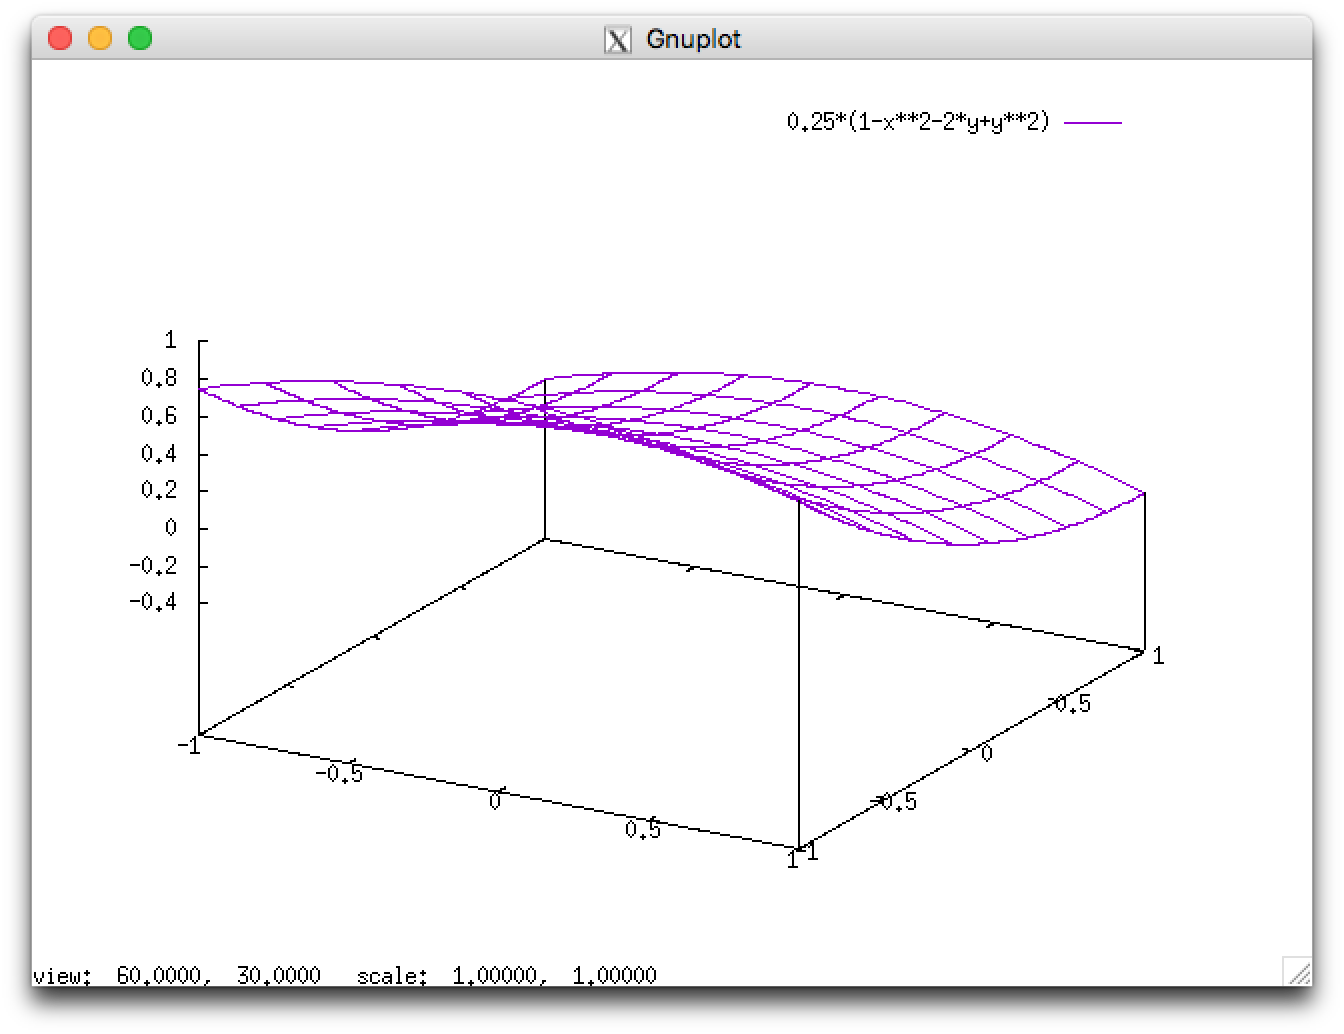
\includegraphics[width=6cm]{images/rannacherturek/N1}
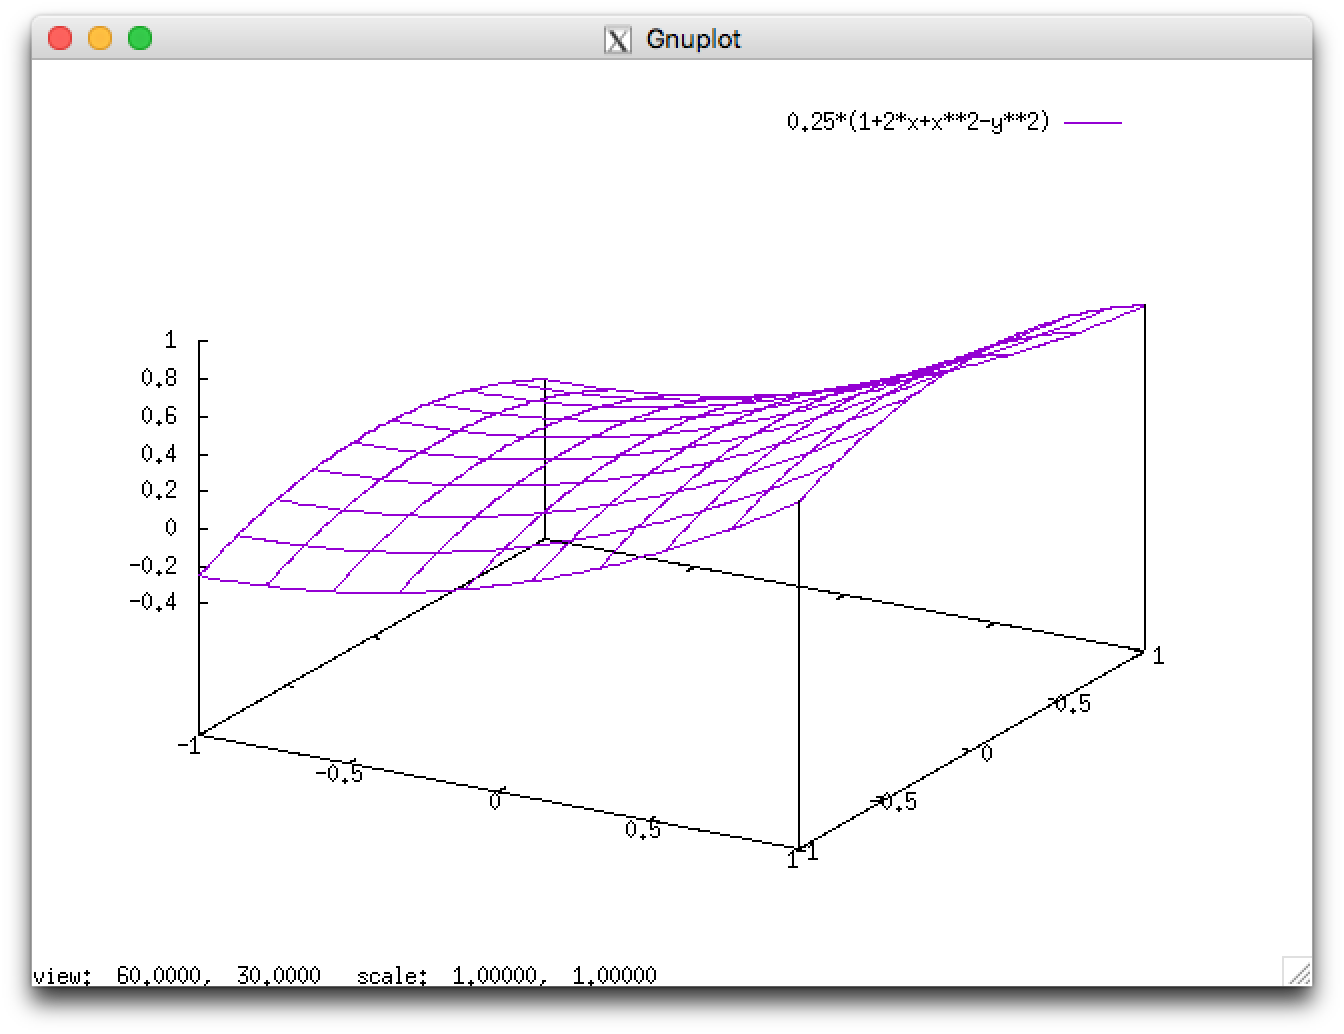
\includegraphics[width=6cm]{images/rannacherturek/N2}\\
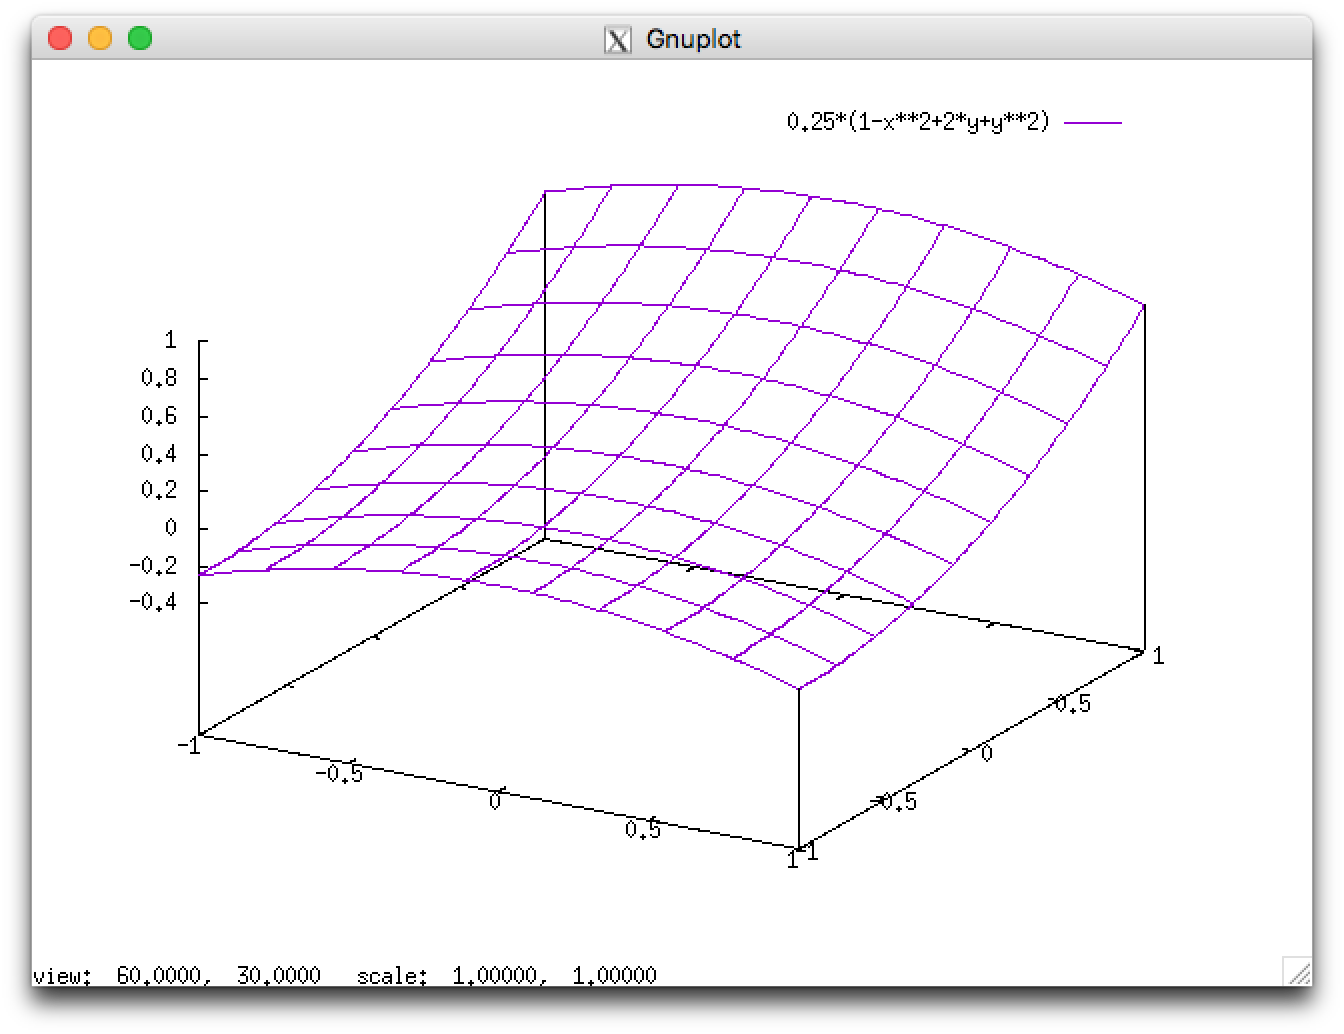
\includegraphics[width=6cm]{images/rannacherturek/N3}
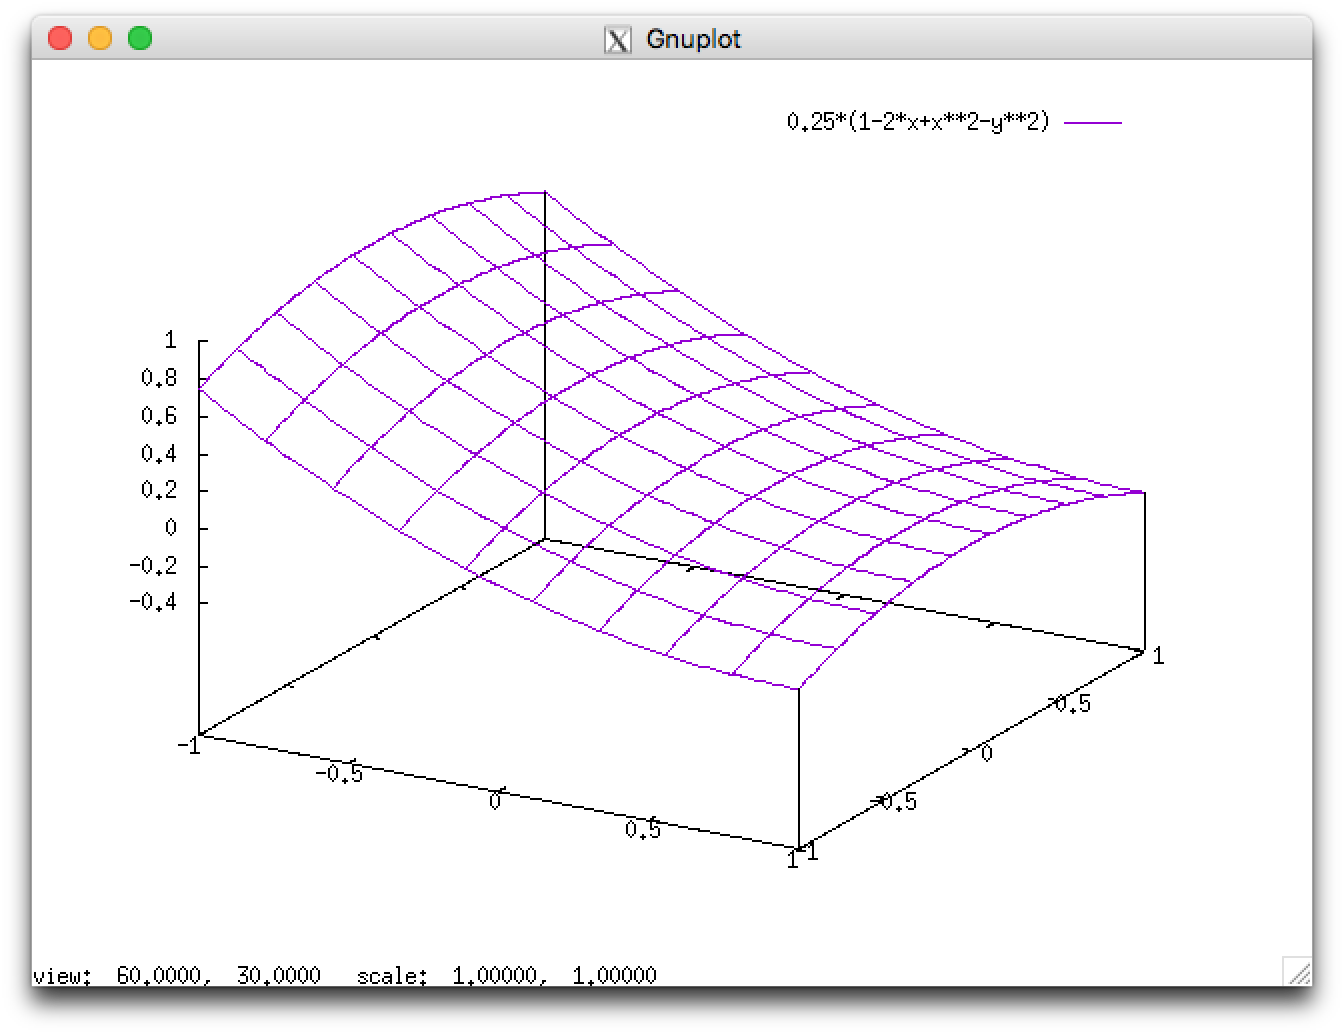
\includegraphics[width=6cm]{images/rannacherturek/N4}\\
{\captionfont Graphical representation of the $\tilde{Q}_1$ shape functions}
\end{center}

%......................................
\paragraph{The Mid Value (MV) variant}. 

These shape functions are implemented in deal.II
\footnote{\url{https://www.dealii.org/8.5.0/doxygen/deal.II/polynomials_rannacher_turek_8cc_source.html}}
for $x\in[0,1]$ and $y\in[0,1]$:

\begin{eqnarray}
N_1(x,y) &=&  0.75 + 1.5x - 2.5y -1.5(x^2-y^2) \quad bottom\\
N_2(x,y) &=& -0.25 - 0.5x + 1.5y +1.5(x^2-y^2) \quad right\\
N_3(x,y) &=& -0.25 + 1.5x - 0.5y -1.5(x^2-y^2) \quad top\\
N_4(x,y) &=&  0.75 - 2.5x + 1.5y +1.5(x^2-y^2) \quad left
\end{eqnarray}
We then proceed to rewrite these for $r\in[-1,1]$ and $t\in[-1:1]$:
\begin{mdframed}[backgroundcolor=blue!5]
\begin{eqnarray}
N_1(r,s) &=& \frac{1}{4} -\frac{1}{2}s - \frac{3}{8}(r^2-s^2) \quad bottom \\
N_2(r,s) &=& \frac{1}{4} +\frac{1}{2}r + \frac{3}{8}(r^2-s^2) \quad right \\
N_3(r,s) &=& \frac{1}{4} +\frac{1}{2}s - \frac{3}{8}(r^2-s^2) \quad top \\
N_4(r,s) &=& \frac{1}{4} -\frac{1}{2}r + \frac{3}{8}(r^2-s^2) \quad left
\end{eqnarray}
\end{mdframed}
It is easy to verify that these functions verify the property
\[
\frac{1}{|\Gamma_i|} \int_{\Gamma_i} N_j d\Gamma = \delta_{ij}
\]

These shape functions are used in \cite{shzh06} and mentioned in John \cite[p.722]{john16}.

\begin{eqnarray}
\frac{\partial N_1}{\partial r} &=& -\frac{3}{4}r \nonumber\\
\frac{\partial N_2}{\partial r} &=& \frac{1}{2}+\frac{3}{4}r \nonumber\\
\frac{\partial N_3}{\partial r} &=& -\frac{3}{4}r \nonumber\\
\frac{\partial N_4}{\partial r} &=& -\frac{1}{2}+\frac{3}{4}r \nonumber
\end{eqnarray}

\begin{eqnarray}
\frac{\partial N_1}{\partial t} &=& -\frac{1}{2}+\frac{3}{4}t \nonumber\\
\frac{\partial N_2}{\partial t} &=& -\frac{3}{4}t \nonumber\\
\frac{\partial N_3}{\partial t} &=& \frac{1}{2}+\frac{3}{4}t \nonumber\\
\frac{\partial N_4}{\partial t} &=& -\frac{3}{4}t \nonumber
\end{eqnarray}



%-----------------------------------------------------------------------------
\subsubsection{The 2D enriched $Q_1^+\times P_0$ of Fortin} \label{ss:Q1pP02D}

\begin{flushright} {\tiny {\color{gray} (tikz\_q1pp02D.tex)}} \end{flushright}
%~~~~~~~~~~~~~~~~~~~~~~~~~~~~~~~~~~~~~~~~~~~~~~~~~~~~~~~~~~~~~~~~~~~~~~~~~~~~~~~~~~~~~~~~~~~~~~~~~~

\begin{center}
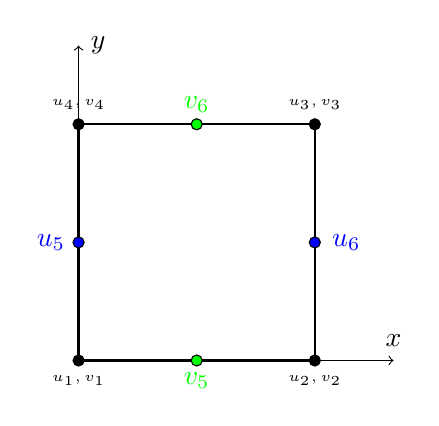
\begin{tikzpicture}
%\draw[fill=gray!23,gray!23](0,0) rectangle (6,5);
%\draw[step=0.5cm,gray,very thin] (0,0) grid (6,5); %background grid

\draw[thick] (1,.5) -- (4,.5) -- (4,3.5) -- (1,3.5) -- cycle; %front

\draw[thin,->] (4,0.5) -- (5,0.5); %x
\draw[thin,->] (1,3.5) -- (1,4.5); %y
\node[] at (5,0.75) {$x$};
\node[] at (1.25,4.5) {$y$};

\draw[black,fill=black] (1,.5)   circle (2pt);
\draw[black,fill=black] (4,.5)   circle (2pt);
\draw[black,fill=black] (4,3.5)   circle (2pt);
\draw[black,fill=black] (1,3.5)   circle (2pt);

\node[] at (1,0.25) {\tiny $u_1,v_1$};
\node[] at (4,0.25) {\tiny $u_2,v_2$};
\node[] at (4,3.75) {\tiny $u_3,v_3$};
\node[] at (1,3.75) {\tiny $u_4,v_4$};

\draw[black,fill=blue] (1,2) circle (2pt); 
\draw[black,fill=blue] (4,2) circle (2pt); 
\node[] at (0.65,2) {\color{blue} $u_5$};
\node[] at (4.4,2) {\color{blue} $u_{6}$};

\draw[black,fill=green] (2.5,0.5) circle (2pt); 
\draw[black,fill=green] (2.5,3.5) circle (2pt); 
\node[] at (2.5,0.25) {\color{green} $v_5$};
\node[] at (2.5,3.75) {\color{green} $v_{6}$};

\end{tikzpicture}\\
\end{center}


\[
u^h(r,s,t) = aN_1 + b N_2 + cN_3 +dN_4 + d b_5(r,s) + e b_{6}(r,s)
\]
with 
\[
b_5^u(r,s) = \frac{1}{2}(1-r)(1-s^2)
\qquad
b_6^u(r,s) = \frac{1}{2}(1+r)(1-s^2)
\]
and
\[
b_5^v(r,s) = \frac{1}{2}(1-r^2)(1-s)
\qquad
b_6^v(r,s) = \frac{1}{2}(1-r^2)(1+s)
\]

\begin{mdframed}[backgroundcolor=blue!5]
\begin{eqnarray}
{N}_1^u(r,s) &=&  N_1(r,s) - \frac{1}{2} b_5^u(r,s)\nn\\
{N}_2^u(r,s) &=&  N_2(r,s) - \frac{1}{2} b_{6}^u(r,s)\nn\\
{N}_3^u(r,s) &=&  N_3(r,s) - \frac{1}{2} b_{6}^u(r,s)\nn\\
{N}_4^u(r,s) &=&  N_4(r,s) - \frac{1}{2} b_5^u(r,s)\nn\\
{N}_5^u(r,s) &=&  b_5^u(r,s)\nn\\
{N}_{6}^u(r,s) &=&  b_{6}^u(r,s) \nn
\end{eqnarray}
\end{mdframed}














